% Options for packages loaded elsewhere
\PassOptionsToPackage{unicode}{hyperref}
\PassOptionsToPackage{hyphens}{url}
%
\documentclass[
]{book}
\usepackage{amsmath,amssymb}
\usepackage{iftex}
\ifPDFTeX
  \usepackage[T1]{fontenc}
  \usepackage[utf8]{inputenc}
  \usepackage{textcomp} % provide euro and other symbols
\else % if luatex or xetex
  \usepackage{unicode-math} % this also loads fontspec
  \defaultfontfeatures{Scale=MatchLowercase}
  \defaultfontfeatures[\rmfamily]{Ligatures=TeX,Scale=1}
\fi
\usepackage{lmodern}
\ifPDFTeX\else
  % xetex/luatex font selection
\fi
% Use upquote if available, for straight quotes in verbatim environments
\IfFileExists{upquote.sty}{\usepackage{upquote}}{}
\IfFileExists{microtype.sty}{% use microtype if available
  \usepackage[]{microtype}
  \UseMicrotypeSet[protrusion]{basicmath} % disable protrusion for tt fonts
}{}
\makeatletter
\@ifundefined{KOMAClassName}{% if non-KOMA class
  \IfFileExists{parskip.sty}{%
    \usepackage{parskip}
  }{% else
    \setlength{\parindent}{0pt}
    \setlength{\parskip}{6pt plus 2pt minus 1pt}}
}{% if KOMA class
  \KOMAoptions{parskip=half}}
\makeatother
\usepackage{xcolor}
\usepackage{color}
\usepackage{fancyvrb}
\newcommand{\VerbBar}{|}
\newcommand{\VERB}{\Verb[commandchars=\\\{\}]}
\DefineVerbatimEnvironment{Highlighting}{Verbatim}{commandchars=\\\{\}}
% Add ',fontsize=\small' for more characters per line
\usepackage{framed}
\definecolor{shadecolor}{RGB}{248,248,248}
\newenvironment{Shaded}{\begin{snugshade}}{\end{snugshade}}
\newcommand{\AlertTok}[1]{\textcolor[rgb]{0.94,0.16,0.16}{#1}}
\newcommand{\AnnotationTok}[1]{\textcolor[rgb]{0.56,0.35,0.01}{\textbf{\textit{#1}}}}
\newcommand{\AttributeTok}[1]{\textcolor[rgb]{0.13,0.29,0.53}{#1}}
\newcommand{\BaseNTok}[1]{\textcolor[rgb]{0.00,0.00,0.81}{#1}}
\newcommand{\BuiltInTok}[1]{#1}
\newcommand{\CharTok}[1]{\textcolor[rgb]{0.31,0.60,0.02}{#1}}
\newcommand{\CommentTok}[1]{\textcolor[rgb]{0.56,0.35,0.01}{\textit{#1}}}
\newcommand{\CommentVarTok}[1]{\textcolor[rgb]{0.56,0.35,0.01}{\textbf{\textit{#1}}}}
\newcommand{\ConstantTok}[1]{\textcolor[rgb]{0.56,0.35,0.01}{#1}}
\newcommand{\ControlFlowTok}[1]{\textcolor[rgb]{0.13,0.29,0.53}{\textbf{#1}}}
\newcommand{\DataTypeTok}[1]{\textcolor[rgb]{0.13,0.29,0.53}{#1}}
\newcommand{\DecValTok}[1]{\textcolor[rgb]{0.00,0.00,0.81}{#1}}
\newcommand{\DocumentationTok}[1]{\textcolor[rgb]{0.56,0.35,0.01}{\textbf{\textit{#1}}}}
\newcommand{\ErrorTok}[1]{\textcolor[rgb]{0.64,0.00,0.00}{\textbf{#1}}}
\newcommand{\ExtensionTok}[1]{#1}
\newcommand{\FloatTok}[1]{\textcolor[rgb]{0.00,0.00,0.81}{#1}}
\newcommand{\FunctionTok}[1]{\textcolor[rgb]{0.13,0.29,0.53}{\textbf{#1}}}
\newcommand{\ImportTok}[1]{#1}
\newcommand{\InformationTok}[1]{\textcolor[rgb]{0.56,0.35,0.01}{\textbf{\textit{#1}}}}
\newcommand{\KeywordTok}[1]{\textcolor[rgb]{0.13,0.29,0.53}{\textbf{#1}}}
\newcommand{\NormalTok}[1]{#1}
\newcommand{\OperatorTok}[1]{\textcolor[rgb]{0.81,0.36,0.00}{\textbf{#1}}}
\newcommand{\OtherTok}[1]{\textcolor[rgb]{0.56,0.35,0.01}{#1}}
\newcommand{\PreprocessorTok}[1]{\textcolor[rgb]{0.56,0.35,0.01}{\textit{#1}}}
\newcommand{\RegionMarkerTok}[1]{#1}
\newcommand{\SpecialCharTok}[1]{\textcolor[rgb]{0.81,0.36,0.00}{\textbf{#1}}}
\newcommand{\SpecialStringTok}[1]{\textcolor[rgb]{0.31,0.60,0.02}{#1}}
\newcommand{\StringTok}[1]{\textcolor[rgb]{0.31,0.60,0.02}{#1}}
\newcommand{\VariableTok}[1]{\textcolor[rgb]{0.00,0.00,0.00}{#1}}
\newcommand{\VerbatimStringTok}[1]{\textcolor[rgb]{0.31,0.60,0.02}{#1}}
\newcommand{\WarningTok}[1]{\textcolor[rgb]{0.56,0.35,0.01}{\textbf{\textit{#1}}}}
\usepackage{longtable,booktabs,array}
\usepackage{calc} % for calculating minipage widths
% Correct order of tables after \paragraph or \subparagraph
\usepackage{etoolbox}
\makeatletter
\patchcmd\longtable{\par}{\if@noskipsec\mbox{}\fi\par}{}{}
\makeatother
% Allow footnotes in longtable head/foot
\IfFileExists{footnotehyper.sty}{\usepackage{footnotehyper}}{\usepackage{footnote}}
\makesavenoteenv{longtable}
\usepackage{graphicx}
\makeatletter
\def\maxwidth{\ifdim\Gin@nat@width>\linewidth\linewidth\else\Gin@nat@width\fi}
\def\maxheight{\ifdim\Gin@nat@height>\textheight\textheight\else\Gin@nat@height\fi}
\makeatother
% Scale images if necessary, so that they will not overflow the page
% margins by default, and it is still possible to overwrite the defaults
% using explicit options in \includegraphics[width, height, ...]{}
\setkeys{Gin}{width=\maxwidth,height=\maxheight,keepaspectratio}
% Set default figure placement to htbp
\makeatletter
\def\fps@figure{htbp}
\makeatother
\setlength{\emergencystretch}{3em} % prevent overfull lines
\providecommand{\tightlist}{%
  \setlength{\itemsep}{0pt}\setlength{\parskip}{0pt}}
\setcounter{secnumdepth}{5}
\usepackage{booktabs}
\usepackage{booktabs}
\usepackage{longtable}
\usepackage{array}
\usepackage{multirow}
\usepackage{wrapfig}
\usepackage{float}
\usepackage{colortbl}
\usepackage{pdflscape}
\usepackage{tabu}
\usepackage{threeparttable}
\usepackage{threeparttablex}
\usepackage[normalem]{ulem}
\usepackage{makecell}
\usepackage{xcolor}
\ifLuaTeX
  \usepackage{selnolig}  % disable illegal ligatures
\fi
\usepackage[]{natbib}
\bibliographystyle{apalike}
\usepackage{bookmark}
\IfFileExists{xurl.sty}{\usepackage{xurl}}{} % add URL line breaks if available
\urlstyle{same}
\hypersetup{
  pdftitle={Atelier sur les méthodes comparées},
  pdfauthor={Simon Joly},
  hidelinks,
  pdfcreator={LaTeX via pandoc}}

\title{Atelier sur les méthodes comparées}
\author{Simon Joly}
\date{2024-11-09}

\begin{document}
\maketitle

{
\setcounter{tocdepth}{1}
\tableofcontents
}
\chapter{À propos}\label{uxe0-propos}

Ce document consiste en une introduction aux méthodes comparatives. Il contient de la théorie ainsi que des exemples pratiques en R sur les moindres carrés phylogénétiques généralisés (PGLS). Il a été développé pour un atelier d'une demi-journée composé de courtes présentations suivies d'exercices R. Notez que le présent document devrait être autonome car la plupart de la théorie donnée dans les présentations est incorporée dans les sections théoriques. Par conséquent, ce document doit contenir toutes les informations nécessaires pour comprendre les exemples.

Je suppose que les lecteurs sont « raisonnablement » familiers avec R ainsi qu'avec la régression linéaire et ses hypothèses. Il existe de nombreux bons didacticiels d'introduction à R sur le Web et pour les modèles linéaires. Zuur et coll. \citep{zuur2007analysing} fournit une bonne introduction aux modèles linéaires, aux modèles à effets mixtes et à la comparaison de modèles. De bonnes introductions à l'ajustement de modèles dans R peuvent également être trouvées sur la {[}page Web{]} de Dolph Schluter (\url{https://www.zoology.ubc.ca/~schluter/R/fit-model/}) et parmi les {[}ateliers QCBS{]} (http~: //qcbs.ca/wiki/r\_workshop4).

\section{Resources utiles}\label{resources-utiles}

Ces liens contiennent des information complémentaires pertinentes.

Le livre de Luke Harmon - \href{https://lukejharmon.github.io/pcm/}{Phylogenetic Comparative Methods}

Le \href{http://blog.phytools.org/}{blog de Liam Revell}

Le livre de Liam Revell et Luke Harmon \href{https://press.princeton.edu/books/ebook/9780691219042/phylogenetic-comparative-methods-in-r}{book on Phylogenetic comparative methods in R}

La liste des \href{https://cran.r-project.org/web/views/Phylogenetics.html}{packages R pour les phylogénies}

\href{http://github.com/simjoly/CourseComparativeMethods/}{Mes tutoriels sur les méthodes comparées}

Le package R \href{https://doi.org/10.1016/j.pld.2022.05.005}{V.PhyloMaker2} qui peut générer de larges phylogénies pour les plantes vasculaires, et le package \href{https://doi.org/10.1016/j.pld.2022.12.007}{U.PhyloMaker} qui peut générer des phylogénies pour les plantes et les animaux.

\section{Source}\label{source}

Ce tutoriel est disponible publiquement et est hébergé sur github dans de dépôt \href{https://github.com/simjoly/AtelierPGLS}{github.com/simjoly/AtelierPGLS}

\section{Disclaimer}\label{disclaimer}

Ce tutoriel est distribué tel quel, avec aucun garantie qu'il va fonctionner ou que les analyses seront à jour.

\chapter{Avant l'atelier}\label{before}

Voici quelques éléments que vous devriez connaître et faire avant l'atelier.

\section{Installer R et les packages requis}\label{installer-r-et-les-packages-requis}

Pour réaliser les exemples de ce document, vous aurez besoin d'avoir le \href{https://www.r-project.org/}{logiciel R} installé sur votre ordinateur. Je vous recommande fortement d'installer \href{https://rstudio.com/}{RStudio}. Bien que R Studio ne soit pas requis, il facilite les interactions entre les scripts et la console R et offre de nombreux outils utiles.

Après avoir installé R, vous devrez installer certains packages. Pour ce tutoriel spécifique, nous devrons charger les packages R suivants.

\begin{Shaded}
\begin{Highlighting}[]
\FunctionTok{library}\NormalTok{(nlme)}
\FunctionTok{library}\NormalTok{(ape)}
\FunctionTok{library}\NormalTok{(RColorBrewer)}
\FunctionTok{library}\NormalTok{(ggplot2)}
\end{Highlighting}
\end{Shaded}

Pour exécuter le code de ce tutoriel dans R, je vous suggère de créer un nouveau script (Fichier\textgreater Nouveau Fichier\textgreater Script R) où vous collerez le code copié depuis les encadrés. Dans R Studio, vous pouvez ensuite exécuter ce code en sélectionnant les lignes que vous souhaitez exécuter puis en appuyant sur ``Run'' (ou le raccourci associé). Cela reproduira les analyses présentées dans le tutoriel. Vous devriez enregistrer le fichier script dans un répertoire dédié pour l'atelier où vous placerez également les fichiers de données requis (voir section \ref{download}). Ensuite, vous devez vous assurer que votre script (et les données) sont dans le répertoire de travail R. Dans R Studio, cela peut être défini via le menu : `Session \textgreater{} Set Working Directory'.

Si certains des packages ci-dessus ne sont pas encore installés sur votre ordinateur, vous recevrez des messages d'erreur lors de leur chargement. Dans ce cas, vous devrez les installer en utilisant la fonction \texttt{install.packages()}. Vous n'avez besoin de les installer qu'une seule fois.

\begin{Shaded}
\begin{Highlighting}[]
\FunctionTok{install.packages}\NormalTok{(}\StringTok{\textquotesingle{}nlme\textquotesingle{}}\NormalTok{)}
\FunctionTok{install.packages}\NormalTok{(}\StringTok{\textquotesingle{}ape\textquotesingle{}}\NormalTok{)}
\FunctionTok{install.packages}\NormalTok{(}\StringTok{\textquotesingle{}RColorBrewer\textquotesingle{}}\NormalTok{)}
\FunctionTok{install.packages}\NormalTok{(}\StringTok{\textquotesingle{}ggplot2\textquotesingle{}}\NormalTok{)}
\end{Highlighting}
\end{Shaded}

Une fois les packages installés, vous pouvez les charger en utilisant la fonction \texttt{library()}. Notez également que si vous utilisez à la fois les packages \texttt{nlme} et \texttt{ape}, \texttt{nlme} doit être chargé en premier. Sinon, vous pourriez rencontrer des erreurs; dans ce cas, vous pouvez redémarrer R et recommencer.

\section{Téléchargement des données}\label{download}

Les données dont vous aurez besoin pour ce tutoriel peuvent être téléchargées depuis ce dépôt : \href{https://simjoly.github.io/ComparativeMethods-HalfDayWorkshop/data.zip}{data.zip}.

Je vous suggère de télécharger le dossier, de le décompresser et de le placer dans un dossier dédié où vous enregistrerez également le script avec toutes les commandes que vous utiliserez.

\section{Familiarisez-vous avec les arbres phylogénétiques dans R}\label{familiarisez-vous-avec-les-arbres-phyloguxe9nuxe9tiques-dans-r}

Si vous n'avez jamais utilisé d'arbres phylogénétiques dans R, vous pouvez apprendre quelques techniques de base pour les manipuler et simuler des arbres et des caractères en lisant le chapitre \ref{trees}.

\chapter{Une introduction aux méthodes comparatives phylogénétiques}\label{intro}

Les méthodes comparatives phylogénétiques ont été introduites par Joseph Felsenstein en 1985. L'idée des méthodes comparatives phylogénétiques était de corriger la non-indépendance des espèces dans les tests statistiques en raison de leurs histoires évolutives partagées. En effet, deux espèces peuvent se ressembler non pas parce qu'elles vivent dans le même environnement mais parce qu'elles sont étroitement liées. Considérez la phylogénie des angiospermes suivante.

\begin{figure}

{\centering 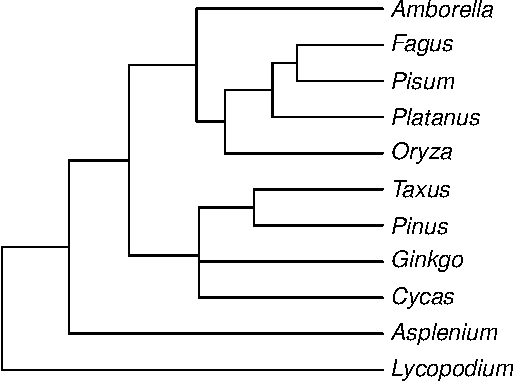
\includegraphics{pcm-workshop_files/figure-latex/AngiospermTree-1} 

}

\caption{land plant phylogeny}\label{fig:AngiospermTree}
\end{figure}

Il est clair que \emph{Fagus} (hêtre) et \emph{Pisum} (pois) sont plus susceptibles de partager des caractéristiques similaires par rapport à \emph{Asplenium} (une fougère), car ils partagent un ancêtre commun plus récent. En d'autres termes, leurs histoires évolutives sont partagées sur une période plus longue qu'avec \emph{Asplenium}. Ainsi, ils ont plus de chances d'avoir des traits plus similaires (et en fait, ils en ont). Par exemple, prenez deux caractères, l'ovule et le type de fécondation, au sein de ce groupe.

\begin{center}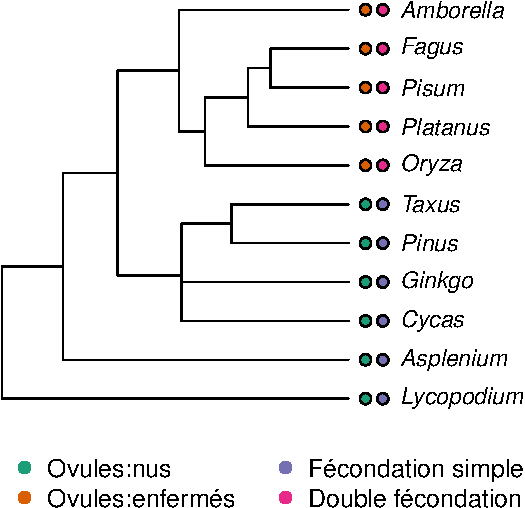
\includegraphics{pcm-workshop_files/figure-latex/AngiospermsWithCharacters-1} \end{center}

En ignorant la phylogénie, nous pourrions être tentés de voir une forte corrélation entre ces deux caractères. En effet, les états entre les deux caractères montrent une correspondance parfaite. En utilisant les statistiques de tableau de contingence standard, nous pourrions faire un test exact de Fisher :

\begin{Shaded}
\begin{Highlighting}[]
\FunctionTok{fisher.test}\NormalTok{(}\FunctionTok{matrix}\NormalTok{(}\FunctionTok{c}\NormalTok{(}\DecValTok{5}\NormalTok{,}\DecValTok{0}\NormalTok{,}\DecValTok{0}\NormalTok{,}\DecValTok{6}\NormalTok{),}\AttributeTok{ncol=}\DecValTok{2}\NormalTok{))}
\end{Highlighting}
\end{Shaded}

\begin{verbatim}
## 
##  Fisher's Exact Test for Count Data
## 
## data:  matrix(c(5, 0, 0, 6), ncol = 2)
## p-value = 0.002165
## alternative hypothesis: true odds ratio is not equal to 1
## 95 percent confidence interval:
##  2.842809      Inf
## sample estimates:
## odds ratio 
##        Inf
\end{verbatim}

Le test suggère que l'association est hautement significative. Cependant, nous savons que les comparaisons faites ne sont pas complètement indépendantes. En réalité, les deux caractères n'ont évolué qu'une seule fois, et ce, le long de la même branche.

Une façon plus appropriée de poser la question serait ``quelle est la probabilité que deux caractères aient évolué le long de la même branche ?''. Cela peut également être calculé en utilisant un tableau de contingence, mais cette fois en prenant les branches de la phylogénie comme unités d'observation.

Dans cet exemple, il y a 18 branches et les deux caractères n'ont évolué qu'une fois et sur la même branche. Le tableau de contingence en considérant les changements le long des branches ressemble à ceci :

\begin{tabular}{>{}l|r|r}
\hline
  & Changement dans le trait 2 & Pas de changement dans le trait 2\\
\hline
\textbf{Changement dans le trait 1} & 1 & 0\\
\hline
\textbf{Pas de changement dans le trait 1} & 0 & 17\\
\hline
\end{tabular}

Avec ce tableau, le test exact de Fisher donnera le résultat suivant :

\begin{Shaded}
\begin{Highlighting}[]
\FunctionTok{fisher.test}\NormalTok{(}\FunctionTok{matrix}\NormalTok{(}\FunctionTok{c}\NormalTok{(}\DecValTok{1}\NormalTok{,}\DecValTok{0}\NormalTok{,}\DecValTok{0}\NormalTok{,}\DecValTok{17}\NormalTok{),}\AttributeTok{ncol=}\DecValTok{2}\NormalTok{))}
\end{Highlighting}
\end{Shaded}

\begin{verbatim}
## 
##  Fisher's Exact Test for Count Data
## 
## data:  matrix(c(1, 0, 0, 17), ncol = 2)
## p-value = 0.05556
## alternative hypothesis: true odds ratio is not equal to 1
## 95 percent confidence interval:
##  0.4358974       Inf
## sample estimates:
## odds ratio 
##        Inf
\end{verbatim}

Vous pouvez voir que le résultat n'est plus significatif.

Bien que cette approche pour prendre en compte les relations phylogénétiques soit correcte, des méthodes comparatives plus puissantes ont été développées. Une approche utile et puissante est le modèle de moindres carrés généralisés phylogénétiques (PGLS). Mais avant d'introduire PGLS, nous allons faire une révision et examiner brièvement la régression standard.

\chapter{Le modèle de régression linéaire}\label{linear-regression}

\section{Théorie}\label{thuxe9orie}

Le modèle linéaire a la forme suivante :

\[\textbf{y} = \alpha + \beta \textbf{x} + \textbf{e}\]

\(\textbf{y}\) est la variable de réponse (ou dépendante), \(\textbf{x}\) est la variable explicative (ou indépendante), et \(\textbf{e}\) représente les résidus ou en d'autres termes la variation non expliquée par le modèle. Pour un modèle de régression linéaire simple, cela représente la distance entre les observations (c'est-à-dire les données réelles) et la ligne de régression (c'est-à-dire la prédiction du modèle) le long de l'axe \(y\). Les paramètres \(\alpha\) représentent l'ordonnée à l'origine, qui es\ldots{}

Obtenir des estimations fiables avec une régression linéaire implique que les données respectent plusieurs hypothèses, parmi lesquelles la normalité, l'homogénéité, \(X\) fixe, l'indépendance et la spécification correcte du modèle. Nous ne passerons pas en revue toutes ces hypothèses ici, mais nous nous concentrerons sur l'une d'entre elles, souvent violée lorsque les données sont structurées phylogénétiquement, qui est \textbf{l'indépendance}. Cette hypothèse est importante car un manque d'indépendance inval\ldots{}

Vous obtenez une violation de l'indépendance lorsque la valeur \(\textbf{y}_i\) à \(\textbf{x}_i\) est influencée par d'autres \(\textbf{x}_i\). Évidemment, cela peut se produire avec des données structurées phylogénétiquement, car une variable de réponse est plus susceptible de réagir de manière similaire chez des espèces étroitement apparentées, car elles partagent de nombreux caractères par filiation. En d'autres termes, la valeur \(y\) d'une espèce n'est pas complètement indépendante de la valeur \(y\) d'un\ldots{}

\section{Pratique}\label{pratique}

Pour fournir des exemples pratiques dans cet atelier, nous utiliserons un jeu de données de traits fonctionnels d'arbres de la province de Québec \citep{paquette2015explaining}. Le jeu de données comprend un certain nombre de traits fonctionnels des plantes et une phylogénie moléculaire construite à l'aide des marqueurs \emph{rbc}L et \emph{mat}K. Le jeu de données dont vous avez besoin pour exécuter les exemples se trouve déjà dans le dossier /data/ du dépôt github. Cependant, vous pouvez également les télécharger en \ldots{}

\href{https://simjoly.github.io/ComparativeMethods-HalfDayWorkshop/data/seedplants.tre}{seedplants.tre}

\href{https://simjoly.github.io/ComparativeMethods-HalfDayWorkshop/data/seedplants.csv}{seedplants.csv}

Avant d'analyser les données, nous commencerons par ouvrir les données et l'arbre phylogénétique et les nettoyer pour ne conserver que les espèces présentes à la fois dans l'arbre et dans le tableau des traits. Cela est nécessaire car certaines espèces supplémentaires ont été incluses dans l'analyse phylogénétique.

\begin{Shaded}
\begin{Highlighting}[]
\FunctionTok{require}\NormalTok{(ape)}
\CommentTok{\# Ouvrir les documents ; cela suppose que vous êtes dans le répertoire principal du dossier de l\textquotesingle{}atelier}
\NormalTok{seedplantstree }\OtherTok{\textless{}{-}} \FunctionTok{read.nexus}\NormalTok{(}\StringTok{"./data/seedplants.tre"}\NormalTok{)}
\NormalTok{seedplantsdata }\OtherTok{\textless{}{-}} \FunctionTok{read.csv2}\NormalTok{(}\StringTok{"./data/seedplants.csv"}\NormalTok{)}
\CommentTok{\# Supprimer les espèces pour lesquelles nous n\textquotesingle{}avons pas de données complètes}
\NormalTok{seedplantsdata }\OtherTok{\textless{}{-}} \FunctionTok{na.omit}\NormalTok{(seedplantsdata)}
\CommentTok{\# Supprimer les espèces de l\textquotesingle{}arbre qui ne sont pas dans la matrice de données}
\NormalTok{species.to.exclude }\OtherTok{\textless{}{-}}\NormalTok{ seedplantstree}\SpecialCharTok{$}\NormalTok{tip.label[}\SpecialCharTok{!}\NormalTok{(seedplantstree}\SpecialCharTok{$}\NormalTok{tip.label }\SpecialCharTok{\%in\%}\NormalTok{ seedplantsdata}\SpecialCharTok{$}\NormalTok{Code)]}
\NormalTok{seedplantstree }\OtherTok{\textless{}{-}} \FunctionTok{drop.tip}\NormalTok{(seedplantstree,species.to.exclude)}
\CommentTok{\# Supprimer l\textquotesingle{}objet inutile}
\FunctionTok{rm}\NormalTok{(species.to.exclude)}
\CommentTok{\# Ordonner l\textquotesingle{}arbre pour qu\textquotesingle{}il soit plus esthétique lors du tracé}
\NormalTok{seedplantstree }\OtherTok{\textless{}{-}} \FunctionTok{ladderize}\NormalTok{(seedplantstree, }\AttributeTok{right =} \ConstantTok{FALSE}\NormalTok{)}
\CommentTok{\# Maintenant, regardons l\textquotesingle{}arbre}
\FunctionTok{plot}\NormalTok{(seedplantstree,}\AttributeTok{cex=}\FloatTok{0.4}\NormalTok{)}
\end{Highlighting}
\end{Shaded}

\begin{center}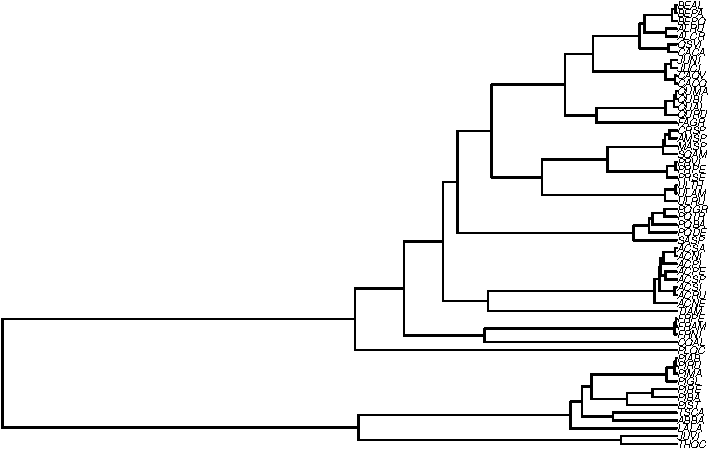
\includegraphics{pcm-workshop_files/figure-latex/Open_seed_plant_data-1} \end{center}

Maintenant, nous pouvons jeter un œil aux données, puis ordonner le trait des plantes pour qu'il soit dans le même ordre que les espèces de l'arbre.

\begin{Shaded}
\begin{Highlighting}[]
\CommentTok{\# Voici à quoi ressemblent les données chargées}
\FunctionTok{head}\NormalTok{(seedplantsdata)}
\end{Highlighting}
\end{Shaded}

\begin{verbatim}
##   Code       Species.name Occurrence maxH   Wd    Sm Shade    N
## 1 ABBA     Abies balsamea       7759   25 0.34   7.6   5.0 1.66
## 2 ACNE       Acer negundo          0   20 0.44  34.0   3.5 2.50
## 3 ACNI        Acer nigrum          1   30 0.52  65.0   3.0 1.83
## 4 ACPE Acer pensylvanicum        665   10 0.44  41.0   3.5 2.22
## 5 ACPL   Acer platanoides          0   15 0.51 172.0   4.2 1.99
## 6 ACRU        Acer rubrum       3669   25 0.49  20.0   3.4 1.91
\end{verbatim}

\begin{Shaded}
\begin{Highlighting}[]
\CommentTok{\# Nommer les lignes du data.frame avec les codes des espèces utilisés comme étiquettes d\textquotesingle{}arbre }
\FunctionTok{rownames}\NormalTok{(seedplantsdata) }\OtherTok{\textless{}{-}}\NormalTok{ seedplantsdata}\SpecialCharTok{$}\NormalTok{Code}
\CommentTok{\# Ordonner les données dans le même ordre que les étiquettes de l\textquotesingle{}arbre. Dans cet exemple }
\CommentTok{\#  précis, c\textquotesingle{}était déjà le cas, mais c\textquotesingle{}est une étape importante pour toute analyse.}
\NormalTok{seedplantsdata }\OtherTok{\textless{}{-}}\NormalTok{ seedplantsdata[seedplantstree}\SpecialCharTok{$}\NormalTok{tip.label,]}
\end{Highlighting}
\end{Shaded}

Maintenant que les données sont prêtes, ajustons un modèle linéaire et essayons d'expliquer la tolérance à l'ombre (Shade) des arbres en utilisant la densité du bois (Wd). En R, une manière très simple de faire une régression est d'utiliser la fonction `lm', qui signifie modèle linéaire. Pour ajuster un modèle linéaire, vous devez dire à la fonction \texttt{lm} quelle variable est la variable de réponse et laquelle est la variable explicative. Cela se fait en utilisant des formules de la forme \texttt{Shade\ \textasciitilde{}\ Wd}. La variab\ldots{}

\begin{Shaded}
\begin{Highlighting}[]
\CommentTok{\# Ajuster un modèle linéaire en utilisant les moindres carrés ordinaires (MCO)}
\NormalTok{shade.lm }\OtherTok{\textless{}{-}} \FunctionTok{lm}\NormalTok{(Shade }\SpecialCharTok{\textasciitilde{}}\NormalTok{ Wd, }\AttributeTok{data =}\NormalTok{ seedplantsdata)}
\CommentTok{\# Imprimer les résultats}
\FunctionTok{summary}\NormalTok{(shade.lm)}
\end{Highlighting}
\end{Shaded}

\begin{verbatim}
## 
## Call:
## lm(formula = Shade ~ Wd, data = seedplantsdata)
## 
## Residuals:
##      Min       1Q   Median       3Q      Max 
## -1.87120 -1.02501  0.05628  0.70132  2.38261 
## 
## Coefficients:
##             Estimate Std. Error t value Pr(>|t|)  
## (Intercept)   2.0010     0.7501   2.668    0.010 *
## Wd            1.8130     1.5676   1.157    0.252  
## ---
## Signif. codes:  0 '***' 0.001 '**' 0.01 '*' 0.05 '.' 0.1 ' ' 1
## 
## Residual standard error: 1.146 on 55 degrees of freedom
## Multiple R-squared:  0.02374,    Adjusted R-squared:  0.005992 
## F-statistic: 1.338 on 1 and 55 DF,  p-value: 0.2525
\end{verbatim}

Vous pouvez voir que l'estimation de la pente (ici le paramètre \texttt{Wd}) est 1.81 et qu'elle n'est pas significative (\(p\)=0.252). Les graphiques descriptifs standards obtenus avec \texttt{plot(shade.lm)} montrent qu'il y a une légère variation plus grande dans les résidus pour les faibles valeurs ajustées, mais elles ne sont pas extrêmes. Cependant, une autre façon de violer l'hypothèse d'indépendance est si les résidus sont corrélés phylog\ldots{}

\begin{Shaded}
\begin{Highlighting}[]
\CommentTok{\# Extraire les résidus}
\NormalTok{shade.res }\OtherTok{\textless{}{-}} \FunctionTok{residuals}\NormalTok{(shade.lm)}

\CommentTok{\#}
\CommentTok{\# Tracer les résidus à côté de la phylogénie}

\CommentTok{\# La commande suivante modifie les paramètres graphiques pour un meilleur rendu de l\textquotesingle{}arbre}
\NormalTok{op }\OtherTok{\textless{}{-}} \FunctionTok{par}\NormalTok{(}\AttributeTok{mar=}\FunctionTok{c}\NormalTok{(}\DecValTok{1}\NormalTok{,}\DecValTok{1}\NormalTok{,}\DecValTok{1}\NormalTok{,}\DecValTok{1}\NormalTok{))}
\CommentTok{\# Vecteur de couleurs pour le tracé de l\textquotesingle{}arbre}
\NormalTok{cols }\OtherTok{\textless{}{-}} \FunctionTok{c}\NormalTok{(}\StringTok{"\#7570b3"}\NormalTok{,}\StringTok{"\#d95f02"}\NormalTok{)}
\CommentTok{\# Les trois commandes suivantes vont tracer l\textquotesingle{}arbre, puis des cercles reflétant }
\CommentTok{\#  les valeurs résiduelles aux extrémités de l\textquotesingle{}arbre, et enfin}
\CommentTok{\#  ajouter une légende.}
\CommentTok{\# La commande plot trace l\textquotesingle{}arbre et laisse un espace pour tracer les }
\CommentTok{\#  résidus aux extrémités avec l\textquotesingle{}option \textquotesingle{}label.offset=0.01\textquotesingle{}}
\FunctionTok{plot}\NormalTok{(seedplantstree,}\AttributeTok{type=}\StringTok{"p"}\NormalTok{,}\ConstantTok{TRUE}\NormalTok{,}\AttributeTok{label.offset=}\FloatTok{0.01}\NormalTok{,}\AttributeTok{cex=}\FloatTok{0.5}\NormalTok{,}\AttributeTok{no.margin=}\ConstantTok{FALSE}\NormalTok{)}
\CommentTok{\# La commande suivante trace les résidus. l\textquotesingle{}option \textquotesingle{}bg\textquotesingle{} est pour la couleur de fond.}
\CommentTok{\#  Si les résidus sont supérieurs à 0 (shade.res\textgreater{}0), il affichera la première couleur}
\CommentTok{\#  (1) du tableau \textquotesingle{}cols\textquotesingle{} et s\textquotesingle{}il est inférieur à zéro, il affiche la deuxième couleur (2). }
\CommentTok{\#  La taille du cercle (l\textquotesingle{}option \textquotesingle{}cex\textquotesingle{}) est relative à la valeur absolue }
\CommentTok{\#  des résidus (abs(shade.res). Pour tracer d\textquotesingle{}autres valeurs, remplacez simplement le }
\CommentTok{\#  vecteur \textquotesingle{}shade.res\textquotesingle{} par un autre.}
\FunctionTok{tiplabels}\NormalTok{(}\AttributeTok{pch=}\DecValTok{21}\NormalTok{,}\AttributeTok{bg=}\NormalTok{cols[}\FunctionTok{ifelse}\NormalTok{(shade.res}\SpecialCharTok{\textgreater{}}\DecValTok{0}\NormalTok{,}\DecValTok{1}\NormalTok{,}\DecValTok{2}\NormalTok{)],}\AttributeTok{col=}\StringTok{"black"}\NormalTok{,}\AttributeTok{cex=}\FunctionTok{abs}\NormalTok{(shade.res),}\AttributeTok{adj=}\FloatTok{0.505}\NormalTok{)}
\CommentTok{\# Imprimer la légende}
\FunctionTok{legend}\NormalTok{(}\StringTok{"topleft"}\NormalTok{,}\AttributeTok{legend=}\FunctionTok{c}\NormalTok{(}\StringTok{"{-}2"}\NormalTok{,}\StringTok{"{-}1"}\NormalTok{,}\StringTok{"0"}\NormalTok{,}\StringTok{"1"}\NormalTok{,}\StringTok{"2"}\NormalTok{),}\AttributeTok{pch=}\DecValTok{21}\NormalTok{,}
       \AttributeTok{pt.bg=}\NormalTok{cols[}\FunctionTok{c}\NormalTok{(}\DecValTok{1}\NormalTok{,}\DecValTok{1}\NormalTok{,}\DecValTok{1}\NormalTok{,}\DecValTok{2}\NormalTok{,}\DecValTok{2}\NormalTok{)],}\AttributeTok{bty=}\StringTok{"n"}\NormalTok{,}
       \AttributeTok{text.col=}\StringTok{"gray32"}\NormalTok{,}\AttributeTok{cex=}\FloatTok{0.8}\NormalTok{,}\AttributeTok{pt.cex=}\FunctionTok{c}\NormalTok{(}\DecValTok{2}\NormalTok{,}\DecValTok{1}\NormalTok{,}\FloatTok{0.1}\NormalTok{,}\DecValTok{1}\NormalTok{,}\DecValTok{2}\NormalTok{))}
\end{Highlighting}
\end{Shaded}

\begin{center}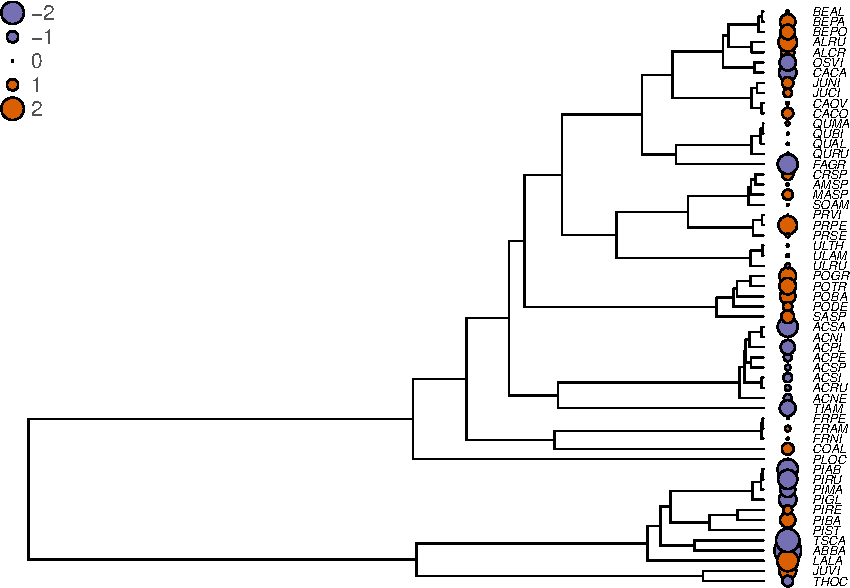
\includegraphics{pcm-workshop_files/figure-latex/Residuals of lm on phylogeny-1} \end{center}

\begin{Shaded}
\begin{Highlighting}[]
\CommentTok{\# Réinitialiser les paramètres graphiques par défaut}
\FunctionTok{par}\NormalTok{(op) }
\end{Highlighting}
\end{Shaded}

Vous pouvez voir que dans plusieurs cas, des espèces étroitement apparentées ont tendance à avoir des résidus similaires (elles sont de la même couleur, ce qui signifie qu'elles sont du même côté de la pente de régression). Cela est problématique. En effet, cela montre que l'hypothèse d'indépendance de la régression des moindres carrés ordinaires (MCO) ne tient plus et les tests statistiques pour les hypothèses nulles ne sont plus valides. Nous verrons ensuite comment les moindres carrés généralisés phylo\ldots{}

\section{Défi no. 1}\label{duxe9fi-no.-1}

Dans le data frame \texttt{seedplantsdata}, il y avait plusieurs traits différents. Essayez d'ajuster une régression de la tolérance à l'ombre des arbres (\texttt{Shade}) en fonction de la masse des graines (\texttt{Sm}). En d'autres termes, testez si la tolérance à l'ombre peut être expliquée par la masse des graines des arbres. Ensuite, essayez de voir si les résidus sont corrélés phylogénétiquement.

\chapter{Phylogenetic generalized least squares (PGLS)}\label{pgls}

\section{Théorie}\label{thuxe9orie-1}

Les moindres carrés généralisés phylogénétiques (PGLS) sont juste une application spécifique de la méthode plus générale appelée moindres carrés généralisés (GLS). Les moindres carrés généralisés relâchent l'hypothèse selon laquelle l'erreur du modèle linéaire doit être non corrélée. Ils permettent à l'utilisateur de spécifier la structure de cette corrélation résiduelle. Cela est utilisé, par exemple, pour corriger la corrélation spatiale, les séries temporelles ou la corrélation phylogénétique.

Les GLS ont la même structure que les Moindres Carrés Ordinaires (OLS)~:

\[\textbf{y} = \alpha + \beta \textbf{x} + \textbf{e}\]

La seule différence est que les résidus sont corrélés entre eux selon une structure de corrélation \(\textbf{C}\) :

\[\textbf{e} \sim N(0,\sigma^2\textbf{C})\]

Ici, \(\textbf{C}\) est une matrice de corrélation qui décrit comment les résidus sont corrélés entre eux. Pour pouvoir tenir compte des relations phylogénétiques dans un PGLS, nous devons donc être capables d'exprimer les relations phylogénétiques sous la forme d'une matrice de corrélation.

\subsection{Structure de corrélation phylogénétique}\label{structure-de-corruxe9lation-phyloguxe9nuxe9tique}

Les relations phylogénétiques peuvent être décrites en utilisant une structure de corrélation. Ci-dessous, vous avez un arbre phylogénétique avec les longueurs de branches indiquées au-dessus des branches.

\begin{flushleft}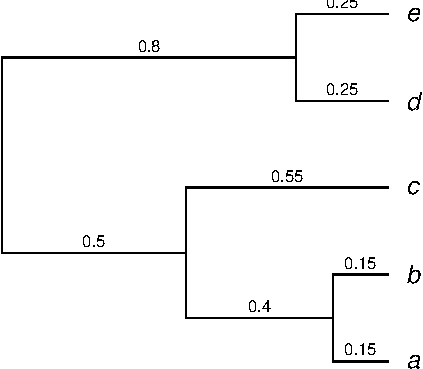
\includegraphics{pcm-workshop_files/figure-latex/phylogenetic tree example-1} \end{flushleft}

Maintenant, cet arbre peut être parfaitement représenté par une matrice de variance-covariance.

\begin{verbatim}
##      a    b    c    d    e
## a 1.05 0.90 0.50 0.00 0.00
## b 0.90 1.05 0.50 0.00 0.00
## c 0.50 0.50 1.05 0.00 0.00
## d 0.00 0.00 0.00 1.05 0.80
## e 0.00 0.00 0.00 0.80 1.05
\end{verbatim}

Les éléments diagonaux de la matrice sont les variances des espèces ; ces nombres représentent la distance totale de la racine de l'arbre aux extrémités. Cela détermine dans quelle mesure les extrémités ont évolué par rapport à la racine. Les éléments hors diagonale sont les covariances entre les espèces. Ils indiquent la proportion du temps pendant laquelle les espèces ont évolué ensemble. Cela correspond à la longueur des branches que deux espèces partagent, à partir de la racine de l'arbre. Par exemple, les espèces \(a\) et \(c\) ont partagé une histoire commune pendant 0,5 unité de temps~; elles ont donc une covariance de 0,5. Plus la covariance est grande, plus les deux espèces ont partagé la même histoire évolutive.

Si toute la variation entre les espèces était due à la phylogénie et non à la sélection, alors cette matrice de variance-covariance représenterait l'attente de la similitude entre toutes les espèces.

\begin{quote}
Notez que toutes les extrémités sont équidistantes de la racine. Lorsque les arbres ont cette propriété, on dit qu'ils sont \textbf{\emph{ultramétriques}}. La plupart des méthodes comparatives phylogénétiques nécessitent que les arbres soient ultramétriques, bien qu'il existe parfois des moyens de relâcher cette hypothèse. Si vous n'avez pas un arbre ultramétrique, il est possible de le rendre ultramétrique en utilisant la fonction chronopl du package ape. Mais idéalement, il est préférable d'utiliser une méthode phylogénétique qui reconstruit directement des arbres ultramétriques.
\end{quote}

La matrice de variance-covariance d'un arbre phylogénétique peut être obtenue à partir d'un arbre en utilisant la fonction vcv du package ape.

\begin{Shaded}
\begin{Highlighting}[]
\CommentTok{\# \textquotesingle{}atree\textquotesingle{} correspond à l\textquotesingle{}arbre phylogénétique montré ci{-}dessus au format newick}
\NormalTok{atree }\OtherTok{\textless{}{-}} \StringTok{"(((a:0.15,b:0.15):0.4,c:0.55):0.5,(d:0.25,e:0.25):0.8);"}
\CommentTok{\# Lisons maintenant cet arbre et stockons{-}le comme un objet d\textquotesingle{}arbre phylogénétique dans R}
\NormalTok{atree }\OtherTok{\textless{}{-}} \FunctionTok{read.tree}\NormalTok{(}\AttributeTok{text=}\NormalTok{atree)}
\CommentTok{\# Afficher l\textquotesingle{}arbre}
\FunctionTok{plot}\NormalTok{(atree)}
\end{Highlighting}
\end{Shaded}

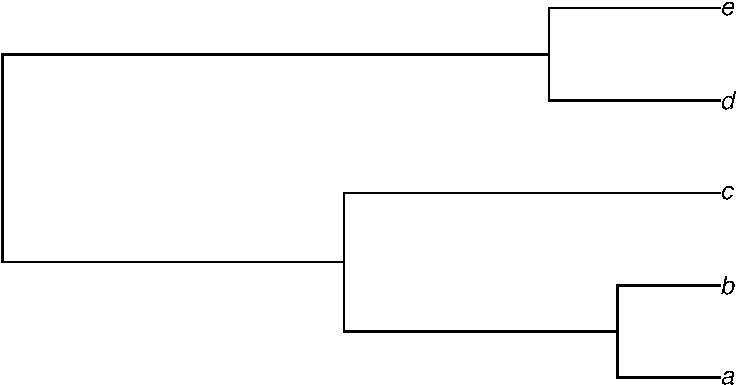
\includegraphics{pcm-workshop_files/figure-latex/vcv function-1.pdf}

\begin{Shaded}
\begin{Highlighting}[]
\CommentTok{\# Extraire la matrice de variance{-}covariance}
\NormalTok{varcovar }\OtherTok{\textless{}{-}} \FunctionTok{vcv}\NormalTok{(atree)}
\CommentTok{\# Imprimer la matrice de variance{-}covariance}
\NormalTok{varcovar}
\end{Highlighting}
\end{Shaded}

\begin{verbatim}
##      a    b    c    d    e
## a 1.05 0.90 0.50 0.00 0.00
## b 0.90 1.05 0.50 0.00 0.00
## c 0.50 0.50 1.05 0.00 0.00
## d 0.00 0.00 0.00 1.05 0.80
## e 0.00 0.00 0.00 0.80 1.05
\end{verbatim}

C'est excellent, mais nous avons mentionné ci-dessus qu'il s'agit d'une matrice de corrélation dont nous avons besoin dans un GLS pour tenir compte de la corrélation dans les résidus. Pour obtenir une matrice de corrélation à partir de la matrice de variance-covariance montrée ci-dessus, il suffit de diviser la matrice de variance-covariance par la longueur de l'arbre, ou la distance de la racine aux extrémités. Elle peut également être obtenue en utilisant la fonction R \texttt{cov2cor}.

\begin{Shaded}
\begin{Highlighting}[]
\CommentTok{\# Convertir la matrice de covariance en une matrice de corrélation}
\NormalTok{corrmat }\OtherTok{\textless{}{-}} \FunctionTok{cov2cor}\NormalTok{(varcovar)}
\CommentTok{\# Imprimer la matrice, arrondie à trois décimales}
\FunctionTok{round}\NormalTok{(corrmat,}\DecValTok{3}\NormalTok{)}
\end{Highlighting}
\end{Shaded}

\begin{verbatim}
##       a     b     c     d     e
## a 1.000 0.857 0.476 0.000 0.000
## b 0.857 1.000 0.476 0.000 0.000
## c 0.476 0.476 1.000 0.000 0.000
## d 0.000 0.000 0.000 1.000 0.762
## e 0.000 0.000 0.000 0.762 1.000
\end{verbatim}

Maintenant, les éléments diagonaux sont égaux à 1, indiquant que les espèces sont parfaitement corrélées avec elles-mêmes. Notez qu'il est également possible d'obtenir directement la matrice de corrélation à partir de la fonction \texttt{vcv} en utilisant l'option \texttt{corr=TRUE}.

\begin{Shaded}
\begin{Highlighting}[]
\CommentTok{\# Obtention d\textquotesingle{}une matrice de corrélation en utilisant la fonction \textquotesingle{}vcv\textquotesingle{}}
\NormalTok{corrmat }\OtherTok{\textless{}{-}} \FunctionTok{vcv}\NormalTok{(atree,}\AttributeTok{corr=}\ConstantTok{TRUE}\NormalTok{)}
\FunctionTok{round}\NormalTok{(corrmat,}\DecValTok{3}\NormalTok{)}
\end{Highlighting}
\end{Shaded}

\begin{verbatim}
##       a     b     c     d     e
## a 1.000 0.857 0.476 0.000 0.000
## b 0.857 1.000 0.476 0.000 0.000
## c 0.476 0.476 1.000 0.000 0.000
## d 0.000 0.000 0.000 1.000 0.762
## e 0.000 0.000 0.000 0.762 1.000
\end{verbatim}

Maintenant que nous savons comment obtenir une matrice de corrélation à partir d'un arbre phylogénétique, nous sommes prêts à exécuter un PGLS.

\section{Défi no. 2}\label{duxe9fi-no.-2}

Pouvez-vous obtenir la matrice de covariance et la matrice de corrélation pour l'arbre phylogénétique des plantes à graines de l'exemple ci-dessus (\texttt{seedplantstree})?

\section{Exercices pratiques}\label{exercices-pratiques}

Il existe plusieurs façons d'exécuter un PGLS en R. Par exemple, le package \texttt{caper} est un package bien connu pour PGLS. Cependant, nous allons utiliser ici la fonction gls du package \texttt{nlme}. Cette fonction est robuste et a l'avantage d'être très flexible. En effet, elle permet d'utiliser facilement des modèles plus complexes tels que les modèles à effets mixtes, bien que cela ne soit pas abordé ici.

Avant d'exécuter le PGLS, exécutons le modèle de base avec la fonction \texttt{gls} comme référence. Exécuter le modèle linéaire standard avec le package nlme permettra d'exécuter des fonctions de comparaison de modèles dans R (voir ci-dessous), ce qui ne serait pas possible si différents modèles étaient ajustés en utilisant différents packages.

\begin{Shaded}
\begin{Highlighting}[]
\FunctionTok{require}\NormalTok{(nlme)}
\NormalTok{shade.pgls0 }\OtherTok{\textless{}{-}} \FunctionTok{gls}\NormalTok{(Shade }\SpecialCharTok{\textasciitilde{}}\NormalTok{ Wd, }\AttributeTok{data =}\NormalTok{ seedplantsdata)}
\FunctionTok{summary}\NormalTok{(shade.pgls0)}
\end{Highlighting}
\end{Shaded}

\begin{verbatim}
## Generalized least squares fit by REML
##   Model: Shade ~ Wd 
##   Data: seedplantsdata 
##       AIC     BIC    logLik
##   180.472 186.494 -87.23602
## 
## Coefficients:
##               Value Std.Error  t-value p-value
## (Intercept) 2.00098 0.7500707 2.667722  0.0100
## Wd          1.81296 1.5675668 1.156544  0.2525
## 
##  Correlation: 
##    (Intr)
## Wd -0.979
## 
## Standardized residuals:
##         Min          Q1         Med          Q3         Max 
## -1.63307700 -0.89457443  0.04911902  0.61207032  2.07940955 
## 
## Residual standard error: 1.145813 
## Degrees of freedom: 57 total; 55 residual
\end{verbatim}

Vous pouvez voir que la sortie est essentiellement identique à celle de la fonction lm. Cependant, il y a quelques différences. L'une est la présence de l'élément « Correlation: » qui donne la corrélation entre les paramètres estimés. De plus, les « résidus standardisés » sont les résidus bruts divisés par l'erreur standard des résidus (les résidus bruts peuvent être affichés avec \texttt{residuals(shade.gls,"response")}).

Maintenant, exécutons un modèle PGLS. Pour attribuer la matrice de corrélation à la fonction \texttt{gls}, il suffit d'utiliser l'option \texttt{corr} de la fonction \texttt{gls}. Cependant, vous devez utiliser une fonction de corrélation spécifique pour que R comprenne qu'il s'agit d'une matrice de corrélation et estime correctement le modèle.

Il existe plusieurs types de structures de corrélation disponibles dans R. Nous commencerons par utiliser l'une des plus simples, appelée \texttt{corSymm}, qui suppose que la matrice de corrélation est symétrique. C'est le cas avec les arbres phylogénétiques; la corrélation entre les espèces \(a\) et \(b\) est la même qu'entre \(b\) et \(a\). Seule la partie triangulaire inférieure de la matrice doit être transmise à la structure corSymm. Si \texttt{mat} est la matrice de corrélation, cela se fait avec la commande \texttt{mat{[}lower.tri(mat){]}}. Ensuite, vous passez la matrice de corrélation à la function \texttt{gls} en utilisant l'argument \texttt{correlation}.

\begin{Shaded}
\begin{Highlighting}[]
\CommentTok{\# Calculer la matrice de corrélation à partir de l\textquotesingle{}arbre}
\NormalTok{mat }\OtherTok{\textless{}{-}} \FunctionTok{vcv}\NormalTok{(seedplantstree,}\AttributeTok{corr=}\ConstantTok{TRUE}\NormalTok{)}
\CommentTok{\# Créer la structure de corrélation pour gls}
\NormalTok{corr.struct }\OtherTok{\textless{}{-}} \FunctionTok{corSymm}\NormalTok{(mat[}\FunctionTok{lower.tri}\NormalTok{(mat)],}\AttributeTok{fixed=}\ConstantTok{TRUE}\NormalTok{)}
\CommentTok{\# Exécuter le pgls}
\NormalTok{shade.pgls1 }\OtherTok{\textless{}{-}} \FunctionTok{gls}\NormalTok{(Shade }\SpecialCharTok{\textasciitilde{}}\NormalTok{ Wd, }\AttributeTok{data =}\NormalTok{ seedplantsdata, }\AttributeTok{correlation=}\NormalTok{corr.struct)}
\FunctionTok{summary}\NormalTok{(shade.pgls1)}
\end{Highlighting}
\end{Shaded}

\begin{verbatim}
## Generalized least squares fit by REML
##   Model: Shade ~ Wd 
##   Data: seedplantsdata 
##        AIC      BIC    logLik
##   214.3762 220.3982 -104.1881
## 
## Correlation Structure: General
##  Formula: ~1 
##  Parameter estimate(s):
##  Correlation: 
##    1     2     3     4     5     6     7     8     9     10    11    12   
## 2  0.000                                                                  
## 3  0.000 0.967                                                            
## 4  0.000 0.967 0.976                                                      
## 5  0.000 0.967 0.981 0.976                                                
## 6  0.000 0.967 0.974 0.974 0.974                                          
## 7  0.000 0.967 0.997 0.976 0.981 0.974                                    
## 8  0.000 0.967 0.974 0.974 0.974 0.997 0.974                              
## 9  0.000 0.967 0.976 0.983 0.976 0.974 0.976 0.974                        
## 10 0.000 0.654 0.654 0.654 0.654 0.654 0.654 0.654 0.654                  
## 11 0.000 0.654 0.654 0.654 0.654 0.654 0.654 0.654 0.654 0.984            
## 12 0.000 0.654 0.654 0.654 0.654 0.654 0.654 0.654 0.654 0.726 0.726      
## 13 0.000 0.654 0.654 0.654 0.654 0.654 0.654 0.654 0.654 0.952 0.952 0.726
## 14 0.000 0.654 0.654 0.654 0.654 0.654 0.654 0.654 0.654 0.952 0.952 0.726
## 15 0.000 0.654 0.654 0.654 0.654 0.654 0.654 0.654 0.654 0.952 0.952 0.726
## 16 0.000 0.654 0.654 0.654 0.654 0.654 0.654 0.654 0.654 0.945 0.945 0.726
## 17 0.000 0.654 0.654 0.654 0.654 0.654 0.654 0.654 0.654 0.876 0.876 0.726
## 18 0.000 0.654 0.654 0.654 0.654 0.654 0.654 0.654 0.654 0.876 0.876 0.726
## 19 0.000 0.596 0.596 0.596 0.596 0.596 0.596 0.596 0.596 0.596 0.596 0.596
## 20 0.000 0.654 0.654 0.654 0.654 0.654 0.654 0.654 0.654 0.726 0.726 0.989
## 21 0.000 0.654 0.654 0.654 0.654 0.654 0.654 0.654 0.654 0.835 0.835 0.726
## 22 0.000 0.596 0.596 0.596 0.596 0.596 0.596 0.596 0.596 0.596 0.596 0.596
## 23 0.000 0.596 0.596 0.596 0.596 0.596 0.596 0.596 0.596 0.596 0.596 0.596
## 24 0.000 0.596 0.596 0.596 0.596 0.596 0.596 0.596 0.596 0.596 0.596 0.596
## 25 0.000 0.654 0.654 0.654 0.654 0.654 0.654 0.654 0.654 0.876 0.876 0.726
## 26 0.000 0.654 0.654 0.654 0.654 0.654 0.654 0.654 0.654 0.876 0.876 0.726
## 27 0.528 0.000 0.000 0.000 0.000 0.000 0.000 0.000 0.000 0.000 0.000 0.000
## 28 0.843 0.000 0.000 0.000 0.000 0.000 0.000 0.000 0.000 0.000 0.000 0.000
## 29 0.000 0.654 0.654 0.654 0.654 0.654 0.654 0.654 0.654 0.726 0.726 0.983
## 30 0.000 0.654 0.654 0.654 0.654 0.654 0.654 0.654 0.654 0.945 0.945 0.726
## 31 0.860 0.000 0.000 0.000 0.000 0.000 0.000 0.000 0.000 0.000 0.000 0.000
## 32 0.860 0.000 0.000 0.000 0.000 0.000 0.000 0.000 0.000 0.000 0.000 0.000
## 33 0.860 0.000 0.000 0.000 0.000 0.000 0.000 0.000 0.000 0.000 0.000 0.000
## 34 0.860 0.000 0.000 0.000 0.000 0.000 0.000 0.000 0.000 0.000 0.000 0.000
## 35 0.860 0.000 0.000 0.000 0.000 0.000 0.000 0.000 0.000 0.000 0.000 0.000
## 36 0.860 0.000 0.000 0.000 0.000 0.000 0.000 0.000 0.000 0.000 0.000 0.000
## 37 0.860 0.000 0.000 0.000 0.000 0.000 0.000 0.000 0.000 0.000 0.000 0.000
## 38 0.000 0.523 0.523 0.523 0.523 0.523 0.523 0.523 0.523 0.523 0.523 0.523
## 39 0.000 0.654 0.654 0.654 0.654 0.654 0.654 0.654 0.654 0.675 0.675 0.675
## 40 0.000 0.654 0.654 0.654 0.654 0.654 0.654 0.654 0.654 0.675 0.675 0.675
## 41 0.000 0.654 0.654 0.654 0.654 0.654 0.654 0.654 0.654 0.675 0.675 0.675
## 42 0.000 0.654 0.654 0.654 0.654 0.654 0.654 0.654 0.654 0.675 0.675 0.675
## 43 0.000 0.654 0.654 0.654 0.654 0.654 0.654 0.654 0.654 0.726 0.726 0.898
## 44 0.000 0.654 0.654 0.654 0.654 0.654 0.654 0.654 0.654 0.726 0.726 0.898
## 45 0.000 0.654 0.654 0.654 0.654 0.654 0.654 0.654 0.654 0.726 0.726 0.898
## 46 0.000 0.654 0.654 0.654 0.654 0.654 0.654 0.654 0.654 0.835 0.835 0.726
## 47 0.000 0.654 0.654 0.654 0.654 0.654 0.654 0.654 0.654 0.835 0.835 0.726
## 48 0.000 0.654 0.654 0.654 0.654 0.654 0.654 0.654 0.654 0.835 0.835 0.726
## 49 0.000 0.654 0.654 0.654 0.654 0.654 0.654 0.654 0.654 0.835 0.835 0.726
## 50 0.000 0.654 0.654 0.654 0.654 0.654 0.654 0.654 0.654 0.675 0.675 0.675
## 51 0.000 0.654 0.654 0.654 0.654 0.654 0.654 0.654 0.654 0.726 0.726 0.980
## 52 0.528 0.000 0.000 0.000 0.000 0.000 0.000 0.000 0.000 0.000 0.000 0.000
## 53 0.000 0.720 0.720 0.720 0.720 0.720 0.720 0.720 0.720 0.654 0.654 0.654
## 54 0.906 0.000 0.000 0.000 0.000 0.000 0.000 0.000 0.000 0.000 0.000 0.000
## 55 0.000 0.654 0.654 0.654 0.654 0.654 0.654 0.654 0.654 0.726 0.726 0.800
## 56 0.000 0.654 0.654 0.654 0.654 0.654 0.654 0.654 0.654 0.726 0.726 0.800
## 57 0.000 0.654 0.654 0.654 0.654 0.654 0.654 0.654 0.654 0.726 0.726 0.800
##    13    14    15    16    17    18    19    20    21    22    23    24   
## 2                                                                         
## 3                                                                         
## 4                                                                         
## 5                                                                         
## 6                                                                         
## 7                                                                         
## 8                                                                         
## 9                                                                         
## 10                                                                        
## 11                                                                        
## 12                                                                        
## 13                                                                        
## 14 0.998                                                                  
## 15 0.994 0.994                                                            
## 16 0.945 0.945 0.945                                                      
## 17 0.876 0.876 0.876 0.876                                                
## 18 0.876 0.876 0.876 0.876 0.998                                          
## 19 0.596 0.596 0.596 0.596 0.596 0.596                                    
## 20 0.726 0.726 0.726 0.726 0.726 0.726 0.596                              
## 21 0.835 0.835 0.835 0.835 0.835 0.835 0.596 0.726                        
## 22 0.596 0.596 0.596 0.596 0.596 0.596 0.715 0.596 0.596                  
## 23 0.596 0.596 0.596 0.596 0.596 0.596 0.715 0.596 0.596 0.997            
## 24 0.596 0.596 0.596 0.596 0.596 0.596 0.715 0.596 0.596 0.999 0.997      
## 25 0.876 0.876 0.876 0.876 0.984 0.984 0.596 0.726 0.835 0.596 0.596 0.596
## 26 0.876 0.876 0.876 0.876 0.984 0.984 0.596 0.726 0.835 0.596 0.596 0.596
## 27 0.000 0.000 0.000 0.000 0.000 0.000 0.000 0.000 0.000 0.000 0.000 0.000
## 28 0.000 0.000 0.000 0.000 0.000 0.000 0.000 0.000 0.000 0.000 0.000 0.000
## 29 0.726 0.726 0.726 0.726 0.726 0.726 0.596 0.983 0.726 0.596 0.596 0.596
## 30 0.945 0.945 0.945 0.988 0.876 0.876 0.596 0.726 0.835 0.596 0.596 0.596
## 31 0.000 0.000 0.000 0.000 0.000 0.000 0.000 0.000 0.000 0.000 0.000 0.000
## 32 0.000 0.000 0.000 0.000 0.000 0.000 0.000 0.000 0.000 0.000 0.000 0.000
## 33 0.000 0.000 0.000 0.000 0.000 0.000 0.000 0.000 0.000 0.000 0.000 0.000
## 34 0.000 0.000 0.000 0.000 0.000 0.000 0.000 0.000 0.000 0.000 0.000 0.000
## 35 0.000 0.000 0.000 0.000 0.000 0.000 0.000 0.000 0.000 0.000 0.000 0.000
## 36 0.000 0.000 0.000 0.000 0.000 0.000 0.000 0.000 0.000 0.000 0.000 0.000
## 37 0.000 0.000 0.000 0.000 0.000 0.000 0.000 0.000 0.000 0.000 0.000 0.000
## 38 0.523 0.523 0.523 0.523 0.523 0.523 0.523 0.523 0.523 0.523 0.523 0.523
## 39 0.675 0.675 0.675 0.675 0.675 0.675 0.596 0.675 0.675 0.596 0.596 0.596
## 40 0.675 0.675 0.675 0.675 0.675 0.675 0.596 0.675 0.675 0.596 0.596 0.596
## 41 0.675 0.675 0.675 0.675 0.675 0.675 0.596 0.675 0.675 0.596 0.596 0.596
## 42 0.675 0.675 0.675 0.675 0.675 0.675 0.596 0.675 0.675 0.596 0.596 0.596
## 43 0.726 0.726 0.726 0.726 0.726 0.726 0.596 0.898 0.726 0.596 0.596 0.596
## 44 0.726 0.726 0.726 0.726 0.726 0.726 0.596 0.898 0.726 0.596 0.596 0.596
## 45 0.726 0.726 0.726 0.726 0.726 0.726 0.596 0.898 0.726 0.596 0.596 0.596
## 46 0.835 0.835 0.835 0.835 0.835 0.835 0.596 0.726 0.881 0.596 0.596 0.596
## 47 0.835 0.835 0.835 0.835 0.835 0.835 0.596 0.726 0.881 0.596 0.596 0.596
## 48 0.835 0.835 0.835 0.835 0.835 0.835 0.596 0.726 0.881 0.596 0.596 0.596
## 49 0.835 0.835 0.835 0.835 0.835 0.835 0.596 0.726 0.881 0.596 0.596 0.596
## 50 0.675 0.675 0.675 0.675 0.675 0.675 0.596 0.675 0.675 0.596 0.596 0.596
## 51 0.726 0.726 0.726 0.726 0.726 0.726 0.596 0.980 0.726 0.596 0.596 0.596
## 52 0.000 0.000 0.000 0.000 0.000 0.000 0.000 0.000 0.000 0.000 0.000 0.000
## 53 0.654 0.654 0.654 0.654 0.654 0.654 0.596 0.654 0.654 0.596 0.596 0.596
## 54 0.000 0.000 0.000 0.000 0.000 0.000 0.000 0.000 0.000 0.000 0.000 0.000
## 55 0.726 0.726 0.726 0.726 0.726 0.726 0.596 0.800 0.726 0.596 0.596 0.596
## 56 0.726 0.726 0.726 0.726 0.726 0.726 0.596 0.800 0.726 0.596 0.596 0.596
## 57 0.726 0.726 0.726 0.726 0.726 0.726 0.596 0.800 0.726 0.596 0.596 0.596
##    25    26    27    28    29    30    31    32    33    34    35    36   
## 2                                                                         
## 3                                                                         
## 4                                                                         
## 5                                                                         
## 6                                                                         
## 7                                                                         
## 8                                                                         
## 9                                                                         
## 10                                                                        
## 11                                                                        
## 12                                                                        
## 13                                                                        
## 14                                                                        
## 15                                                                        
## 16                                                                        
## 17                                                                        
## 18                                                                        
## 19                                                                        
## 20                                                                        
## 21                                                                        
## 22                                                                        
## 23                                                                        
## 24                                                                        
## 25                                                                        
## 26 0.992                                                                  
## 27 0.000 0.000                                                            
## 28 0.000 0.000 0.528                                                      
## 29 0.726 0.726 0.000 0.000                                                
## 30 0.876 0.876 0.000 0.000 0.726                                          
## 31 0.000 0.000 0.528 0.843 0.000 0.000                                    
## 32 0.000 0.000 0.528 0.843 0.000 0.000 0.874                              
## 33 0.000 0.000 0.528 0.843 0.000 0.000 0.985 0.874                        
## 34 0.000 0.000 0.528 0.843 0.000 0.000 0.997 0.874 0.985                  
## 35 0.000 0.000 0.528 0.843 0.000 0.000 0.874 0.965 0.874 0.874            
## 36 0.000 0.000 0.528 0.843 0.000 0.000 0.999 0.874 0.985 0.997 0.874      
## 37 0.000 0.000 0.528 0.843 0.000 0.000 0.874 0.926 0.874 0.874 0.926 0.874
## 38 0.523 0.523 0.000 0.000 0.523 0.523 0.000 0.000 0.000 0.000 0.000 0.000
## 39 0.675 0.675 0.000 0.000 0.675 0.675 0.000 0.000 0.000 0.000 0.000 0.000
## 40 0.675 0.675 0.000 0.000 0.675 0.675 0.000 0.000 0.000 0.000 0.000 0.000
## 41 0.675 0.675 0.000 0.000 0.675 0.675 0.000 0.000 0.000 0.000 0.000 0.000
## 42 0.675 0.675 0.000 0.000 0.675 0.675 0.000 0.000 0.000 0.000 0.000 0.000
## 43 0.726 0.726 0.000 0.000 0.898 0.726 0.000 0.000 0.000 0.000 0.000 0.000
## 44 0.726 0.726 0.000 0.000 0.898 0.726 0.000 0.000 0.000 0.000 0.000 0.000
## 45 0.726 0.726 0.000 0.000 0.898 0.726 0.000 0.000 0.000 0.000 0.000 0.000
## 46 0.835 0.835 0.000 0.000 0.726 0.835 0.000 0.000 0.000 0.000 0.000 0.000
## 47 0.835 0.835 0.000 0.000 0.726 0.835 0.000 0.000 0.000 0.000 0.000 0.000
## 48 0.835 0.835 0.000 0.000 0.726 0.835 0.000 0.000 0.000 0.000 0.000 0.000
## 49 0.835 0.835 0.000 0.000 0.726 0.835 0.000 0.000 0.000 0.000 0.000 0.000
## 50 0.675 0.675 0.000 0.000 0.675 0.675 0.000 0.000 0.000 0.000 0.000 0.000
## 51 0.726 0.726 0.000 0.000 0.980 0.726 0.000 0.000 0.000 0.000 0.000 0.000
## 52 0.000 0.000 0.918 0.528 0.000 0.000 0.528 0.528 0.528 0.528 0.528 0.528
## 53 0.654 0.654 0.000 0.000 0.654 0.654 0.000 0.000 0.000 0.000 0.000 0.000
## 54 0.000 0.000 0.528 0.843 0.000 0.000 0.860 0.860 0.860 0.860 0.860 0.860
## 55 0.726 0.726 0.000 0.000 0.800 0.726 0.000 0.000 0.000 0.000 0.000 0.000
## 56 0.726 0.726 0.000 0.000 0.800 0.726 0.000 0.000 0.000 0.000 0.000 0.000
## 57 0.726 0.726 0.000 0.000 0.800 0.726 0.000 0.000 0.000 0.000 0.000 0.000
##    37    38    39    40    41    42    43    44    45    46    47    48   
## 2                                                                         
## 3                                                                         
## 4                                                                         
## 5                                                                         
## 6                                                                         
## 7                                                                         
## 8                                                                         
## 9                                                                         
## 10                                                                        
## 11                                                                        
## 12                                                                        
## 13                                                                        
## 14                                                                        
## 15                                                                        
## 16                                                                        
## 17                                                                        
## 18                                                                        
## 19                                                                        
## 20                                                                        
## 21                                                                        
## 22                                                                        
## 23                                                                        
## 24                                                                        
## 25                                                                        
## 26                                                                        
## 27                                                                        
## 28                                                                        
## 29                                                                        
## 30                                                                        
## 31                                                                        
## 32                                                                        
## 33                                                                        
## 34                                                                        
## 35                                                                        
## 36                                                                        
## 37                                                                        
## 38 0.000                                                                  
## 39 0.000 0.523                                                            
## 40 0.000 0.523 0.959                                                      
## 41 0.000 0.523 0.964 0.959                                                
## 42 0.000 0.523 0.964 0.959 0.982                                          
## 43 0.000 0.523 0.675 0.675 0.675 0.675                                    
## 44 0.000 0.523 0.675 0.675 0.675 0.675 0.986                              
## 45 0.000 0.523 0.675 0.675 0.675 0.675 0.998 0.986                        
## 46 0.000 0.523 0.675 0.675 0.675 0.675 0.726 0.726 0.726                  
## 47 0.000 0.523 0.675 0.675 0.675 0.675 0.726 0.726 0.726 0.997            
## 48 0.000 0.523 0.675 0.675 0.675 0.675 0.726 0.726 0.726 0.997 0.999      
## 49 0.000 0.523 0.675 0.675 0.675 0.675 0.726 0.726 0.726 0.984 0.984 0.984
## 50 0.000 0.523 0.936 0.936 0.936 0.936 0.675 0.675 0.675 0.675 0.675 0.675
## 51 0.000 0.523 0.675 0.675 0.675 0.675 0.898 0.898 0.898 0.726 0.726 0.726
## 52 0.528 0.000 0.000 0.000 0.000 0.000 0.000 0.000 0.000 0.000 0.000 0.000
## 53 0.000 0.523 0.654 0.654 0.654 0.654 0.654 0.654 0.654 0.654 0.654 0.654
## 54 0.860 0.000 0.000 0.000 0.000 0.000 0.000 0.000 0.000 0.000 0.000 0.000
## 55 0.000 0.523 0.675 0.675 0.675 0.675 0.800 0.800 0.800 0.726 0.726 0.726
## 56 0.000 0.523 0.675 0.675 0.675 0.675 0.800 0.800 0.800 0.726 0.726 0.726
## 57 0.000 0.523 0.675 0.675 0.675 0.675 0.800 0.800 0.800 0.726 0.726 0.726
##    49    50    51    52    53    54    55    56   
## 2                                                 
## 3                                                 
## 4                                                 
## 5                                                 
## 6                                                 
## 7                                                 
## 8                                                 
## 9                                                 
## 10                                                
## 11                                                
## 12                                                
## 13                                                
## 14                                                
## 15                                                
## 16                                                
## 17                                                
## 18                                                
## 19                                                
## 20                                                
## 21                                                
## 22                                                
## 23                                                
## 24                                                
## 25                                                
## 26                                                
## 27                                                
## 28                                                
## 29                                                
## 30                                                
## 31                                                
## 32                                                
## 33                                                
## 34                                                
## 35                                                
## 36                                                
## 37                                                
## 38                                                
## 39                                                
## 40                                                
## 41                                                
## 42                                                
## 43                                                
## 44                                                
## 45                                                
## 46                                                
## 47                                                
## 48                                                
## 49                                                
## 50 0.675                                          
## 51 0.726 0.675                                    
## 52 0.000 0.000 0.000                              
## 53 0.654 0.654 0.654 0.000                        
## 54 0.000 0.000 0.000 0.528 0.000                  
## 55 0.726 0.675 0.800 0.000 0.654 0.000            
## 56 0.726 0.675 0.800 0.000 0.654 0.000 0.983      
## 57 0.726 0.675 0.800 0.000 0.654 0.000 0.999 0.983
## 
## Coefficients:
##                Value Std.Error   t-value p-value
## (Intercept) 0.911433  4.409058 0.2067184  0.8370
## Wd          4.361028  1.693349 2.5753865  0.0127
## 
##  Correlation: 
##    (Intr)
## Wd -0.166
## 
## Standardized residuals:
##         Min          Q1         Med          Q3         Max 
## -0.26890642 -0.16431866 -0.02645422  0.09638984  0.34953444 
## 
## Residual standard error: 7.455109 
## Degrees of freedom: 57 total; 55 residual
\end{verbatim}

Notez que le terme \texttt{fixed=TRUE} dans la structure corSymm indique que la structure de corrélation est fixée pendant l'optimisation des paramètres.

La sortie est similaire à celle du modèle sans corrélation, sauf pour la sortie de la matrice de corrélation.

Fait intéressant, vous pouvez voir que l'estimation du coefficient pour la pente est plus grande (4.361) qu'avec la régression standard et également significative (\(p\)=0.0127). C'est un exemple positif de PGLS. En effet, la relation entre la tolérance à l'ombre et la densité du bois était obscurcie par la corrélation phylogénétique des résidus. Une fois cette corrélation prise en compte, la relation significative est révélée.

Une relation significative entre la tolérance à l'ombre et la densité du bois a en fait un sens, bien que cette relation ne soit probablement pas causale. En effet, les arbres tolérants à l'ombre sont généralement des espèces de succession et poussent souvent plus lentement, en partie à cause de la disponibilité limitée de la lumière, et ont donc tendance à développer des bois de densité plus élevée.

Maintenant, regardons les résidus du modèle. Pour extraire les résidus corrigés par la structure de corrélation, vous devez demander les résidus normalisés.

\begin{Shaded}
\begin{Highlighting}[]
\CommentTok{\# Extraire les résidus corrigés par la structure de corrélation}
\NormalTok{pgls1.res }\OtherTok{\textless{}{-}} \FunctionTok{residuals}\NormalTok{(shade.pgls1,}\AttributeTok{type=}\StringTok{"normalized"}\NormalTok{)}
\CommentTok{\# Modifier les paramètres graphiques}
\NormalTok{op }\OtherTok{\textless{}{-}} \FunctionTok{par}\NormalTok{(}\AttributeTok{mar=}\FunctionTok{c}\NormalTok{(}\DecValTok{1}\NormalTok{,}\DecValTok{1}\NormalTok{,}\DecValTok{1}\NormalTok{,}\DecValTok{1}\NormalTok{))}
\CommentTok{\# Même tracé que ci{-}dessus sauf pour utiliser pgls1.res comme résidus}
\FunctionTok{plot}\NormalTok{(seedplantstree,}\AttributeTok{type=}\StringTok{"p"}\NormalTok{,}\ConstantTok{TRUE}\NormalTok{,}\AttributeTok{label.offset=}\FloatTok{0.01}\NormalTok{,}\AttributeTok{cex=}\FloatTok{0.5}\NormalTok{,}\AttributeTok{no.margin=}\ConstantTok{FALSE}\NormalTok{)}
\FunctionTok{tiplabels}\NormalTok{(}\AttributeTok{pch=}\DecValTok{21}\NormalTok{,}\AttributeTok{bg=}\NormalTok{cols[}\FunctionTok{ifelse}\NormalTok{(pgls1.res}\SpecialCharTok{\textgreater{}}\DecValTok{0}\NormalTok{,}\DecValTok{1}\NormalTok{,}\DecValTok{2}\NormalTok{)],}\AttributeTok{col=}\StringTok{"black"}\NormalTok{,}
          \AttributeTok{cex=}\FunctionTok{abs}\NormalTok{(pgls1.res),}\AttributeTok{adj=}\FloatTok{0.505}\NormalTok{)}
\FunctionTok{legend}\NormalTok{(}\StringTok{"topleft"}\NormalTok{,}\AttributeTok{legend=}\FunctionTok{c}\NormalTok{(}\StringTok{"{-}2"}\NormalTok{,}\StringTok{"{-}1"}\NormalTok{,}\StringTok{"0"}\NormalTok{,}\StringTok{"1"}\NormalTok{,}\StringTok{"2"}\NormalTok{),}\AttributeTok{pch=}\DecValTok{21}\NormalTok{,}
       \AttributeTok{pt.bg=}\NormalTok{cols[}\FunctionTok{c}\NormalTok{(}\DecValTok{1}\NormalTok{,}\DecValTok{1}\NormalTok{,}\DecValTok{1}\NormalTok{,}\DecValTok{2}\NormalTok{,}\DecValTok{2}\NormalTok{)],}\AttributeTok{bty=}\StringTok{"n"}\NormalTok{,}
       \AttributeTok{text.col=}\StringTok{"black"}\NormalTok{,}\AttributeTok{cex=}\FloatTok{0.8}\NormalTok{,}\AttributeTok{pt.cex=}\FunctionTok{c}\NormalTok{(}\DecValTok{2}\NormalTok{,}\DecValTok{1}\NormalTok{,}\FloatTok{0.1}\NormalTok{,}\DecValTok{1}\NormalTok{,}\DecValTok{2}\NormalTok{))}
\end{Highlighting}
\end{Shaded}

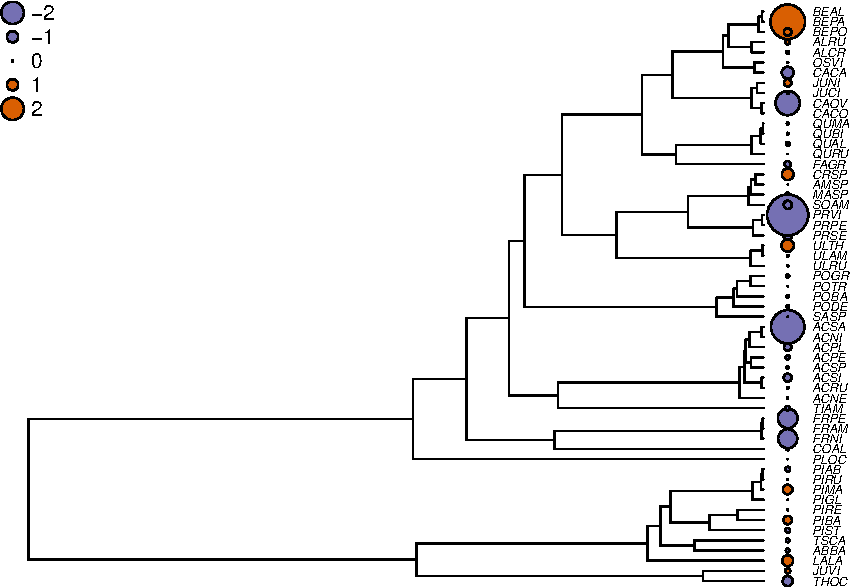
\includegraphics{pcm-workshop_files/figure-latex/pgls residual fit-1.pdf}

\begin{Shaded}
\begin{Highlighting}[]
\CommentTok{\# Réinitialiser les paramètres graphiques par défaut}
\FunctionTok{par}\NormalTok{(op)}
\end{Highlighting}
\end{Shaded}

Si vous comparez avec l'optimisation des moindres carrés ordinaires, les résidus sont beaucoup moins corrélés phylogénétiquement.

\subsection{Autres structures de corrélation}\label{autres-structures-de-corruxe9lation}

Dans le PGLS précédent, nous avons utilisé la structure corSymm pour transmettre la structure de corrélation phylogénétique à gls. Cela fonctionne parfaitement, mais il existe des moyens plus simples. Julien Dutheil a développé des structures phylogénétiques à utiliser spécialement dans les PGLS.

Celui que nous avons utilisé ci-dessus est équivalent à la structure \texttt{corBrownian} de \texttt{ape}. Cette approche est plus simple et il suffit de transmettre l'arbre à la structure de corrélation. Voici le même exemple en utilisant la structure \texttt{corBrownian}.

\begin{Shaded}
\begin{Highlighting}[]
\CommentTok{\# Obtenir la structure de corrélation}
\NormalTok{bm.corr }\OtherTok{\textless{}{-}} \FunctionTok{corBrownian}\NormalTok{(}\AttributeTok{phy=}\NormalTok{seedplantstree, }\AttributeTok{form=}\SpecialCharTok{\textasciitilde{}}\DecValTok{1}\NormalTok{)}
\CommentTok{\# PGLS}
\NormalTok{shade.pgls1b }\OtherTok{\textless{}{-}} \FunctionTok{gls}\NormalTok{(Shade }\SpecialCharTok{\textasciitilde{}}\NormalTok{ Wd, }\AttributeTok{data =}\NormalTok{ seedplantsdata, }\AttributeTok{correlation=}\NormalTok{bm.corr)}
\end{Highlighting}
\end{Shaded}

\begin{verbatim}
## Warning in Initialize.corPhyl(X[[i]], ...): No covariate specified, species
## will be taken as ordered in the data frame. To avoid this message, specify a
## covariate containing the species names with the 'form' argument.
\end{verbatim}

\begin{Shaded}
\begin{Highlighting}[]
\FunctionTok{summary}\NormalTok{(shade.pgls1b)}
\end{Highlighting}
\end{Shaded}

\begin{verbatim}
## Generalized least squares fit by REML
##   Model: Shade ~ Wd 
##   Data: seedplantsdata 
##        AIC      BIC    logLik
##   214.3762 220.3982 -104.1881
## 
## Correlation Structure: corBrownian
##  Formula: ~1 
##  Parameter estimate(s):
## numeric(0)
## 
## Coefficients:
##                Value Std.Error   t-value p-value
## (Intercept) 0.911433  4.409058 0.2067184  0.8370
## Wd          4.361028  1.693349 2.5753865  0.0127
## 
##  Correlation: 
##    (Intr)
## Wd -0.166
## 
## Standardized residuals:
##         Min          Q1         Med          Q3         Max 
## -0.26890642 -0.16431866 -0.02645422  0.09638984  0.34953444 
## 
## Residual standard error: 7.455109 
## Degrees of freedom: 57 total; 55 residual
\end{verbatim}

Vous pouvez voir que les résultats sont identiques. La seule différence est que la structure de corrélation n'est pas affichée dans le résumé. Le \texttt{numeric(0)} signifie qu'aucun paramètre n'a été estimé pendant l'optimisation (il et fixe).

Maintenant, vous vous demandez peut-être pourquoi la structure de corrélation ets appelée corBrownian. C'est parce qu'elle utilise le mouvement Brownien pour modéliser l'évolution le long des branches de l'arbre. Ce processus est souvent référé comme un modèle neutre. Si vous voulez en savoir davantage du le modèle Brownien, vous pouvez lire la section \ref{BM-model} à propos de ce modèle.

\section{Défi no. 3}\label{duxe9fi-no.-3}

Ajuster un modèle PGLS pour voir si le poids des graines (\texttt{Sm}) explique la tolérance à l'ombre (\texttt{Shade}) à l'aide du jeu de données seedplantdataset. Comment est-ce que ces résultats se comparent avec les résultats d'une régression standard.

\chapter{Contrastes Indépendants Phylogénétiques}\label{pic}

Faisons une digression pour examiner les Contrastes Indépendants Phylogénétiques (PIC). Les PIC ont été la première approche comparative proposée pour traiter la non-indépendance phylogénétique \citep{felsenstein1985phylogenies}. Bien qu'ils soient moins flexibles que les PGLS, ils donnent les mêmes résultats. Voyons comment ils peuvent être utilisés.

Les contrastes indépendants phylogénétiques sont estimés un trait à la fois. Ils transforment essentiellement le trait observé en contrastes qui ne sont pas corrélés avec la phylogénie. Cela peut être fait dans R en utilisant la fonction \texttt{pic} du package \texttt{ape}.

\begin{Shaded}
\begin{Highlighting}[]
\CommentTok{\# Estimer le PIC pour la tolérance à l\textquotesingle{}ombre }
\NormalTok{Shade.pic }\OtherTok{\textless{}{-}} \FunctionTok{pic}\NormalTok{(seedplantsdata}\SpecialCharTok{$}\NormalTok{Shade, }\AttributeTok{phy=}\NormalTok{seedplantstree)}
\CommentTok{\# Estimer le PIC pour la densité du bois }
\NormalTok{Wd.pic }\OtherTok{\textless{}{-}} \FunctionTok{pic}\NormalTok{(seedplantsdata}\SpecialCharTok{$}\NormalTok{Wd, }\AttributeTok{phy=}\NormalTok{seedplantstree)}
\end{Highlighting}
\end{Shaded}

Une fois cela fait, il suffit d'ajuster une régression entre ces contrastes. Notez qu'il est important que l'ordonnée à l'origine soit fixée à 0 dans le modèle. Cela se fait en ajoutant \texttt{-\ 1} à droite de la formule.

\begin{Shaded}
\begin{Highlighting}[]
\CommentTok{\# Estimer le PIC pour la tolérance à l\textquotesingle{}ombre }
\NormalTok{pic.results }\OtherTok{\textless{}{-}} \FunctionTok{lm}\NormalTok{(Shade.pic }\SpecialCharTok{\textasciitilde{}}\NormalTok{ Wd.pic }\SpecialCharTok{{-}} \DecValTok{1}\NormalTok{)}
\FunctionTok{summary}\NormalTok{(pic.results)}
\end{Highlighting}
\end{Shaded}

\begin{verbatim}
## 
## Call:
## lm(formula = Shade.pic ~ Wd.pic - 1)
## 
## Residuals:
##     Min      1Q  Median      3Q     Max 
## -71.943  -4.106   1.013   5.679  21.614 
## 
## Coefficients:
##        Estimate Std. Error t value Pr(>|t|)  
## Wd.pic    4.361      1.693   2.575   0.0127 *
## ---
## Signif. codes:  0 '***' 0.001 '**' 0.01 '*' 0.05 '.' 0.1 ' ' 1
## 
## Residual standard error: 19.21 on 55 degrees of freedom
## Multiple R-squared:  0.1076, Adjusted R-squared:  0.09139 
## F-statistic: 6.633 on 1 and 55 DF,  p-value: 0.01273
\end{verbatim}

Vous pouvez voir que l'estimation de la pente, \texttt{4.361}, est identique à celle obtenue avec les PGLS. Même chose pour la valeur p.~La principale limitation des PIC est que vous êtes limité à toujours comparer deux variables. Avec les PGLS, une flexibilité beaucoup plus grande est possible.

\chapter{Assouplir l'hypothèse selon laquelle les résidus doivent être parfaitement corrélés phylogénétiquement}\label{assouplir-lhypothuxe8se-selon-laquelle-les-ruxe9sidus-doivent-uxeatre-parfaitement-corruxe9luxe9s-phyloguxe9nuxe9tiquement}

Les moindres carrés généralisés phylogénétiques supposent que les résidus sont parfaitement corrélés phylogénétiquement. Cela est relativement contraignant car cela signifie que d'autres sources d'erreurs non corrélées phylogénétiquement ne sont pas autorisées par le modèle. De plus, si elles existent, elles peuvent biaiser les résultats des PGLS \citep{revell2010phylogenetic}.

Il existe des moyens d'assouplir cette hypothèse, et l'un d'eux consiste à utiliser un type de structure de corrélation qui permet cet assouplissement.

\section{Théorie : Structure de corrélation de Pagel}\label{thuxe9orie-structure-de-corruxe9lation-de-pagel}

Lors du contrôle des relations phylogénétiques avec les moindres carrés généralisés phylogénétiques, nous supposons que les résidus sont parfaitement corrélés en fonction de la structure de corrélation. En pratique, ce n'est pas toujours le cas, et il est difficile de vraiment savoir à quel point il est important de contrôler la relation phylogénétique dans un cas spécifique. Par exemple, pour une étude donnée, la corrélation dans les résidus peut ne pas être fortement corrélée phylogénétiquement.

Il est possible de prendre cela en compte en utilisant le modèle \(\lambda\) de Pagel \citep{pagel1999inferring}. L'idée est de multiplier les éléments hors diagonale de la matrice de corrélation (essentiellement les longueurs de branches de la phylogénie) par un paramètre \(\lambda\), mais pas les valeurs diagonales. Cela entraîne essentiellement une modification des longueurs de branches de la phylogénie. Une valeur de \(\lambda\) proche de zéro donne des branches internes très courtes et de longues branches terminales. Cela réduit, en effet, les corrélations phylogénétiques (l'effet de la phylogénie est réduit). À l'opposé, si \(\lambda\) est proche de 1, alors la phylogénie modifiée ressemble à la phylogénie réelle. En effet, le paramètre \(\lambda\) est souvent interprété comme un paramètre de signal phylogénétique~; ainsi, une valeur de \(\lambda\) plus élevée implique un signal phylogénétique plus fort.

La figure suivante montre comment différentes valeurs de lambda affectent la forme de la phylogénie des arbres du Québec.

\begin{center}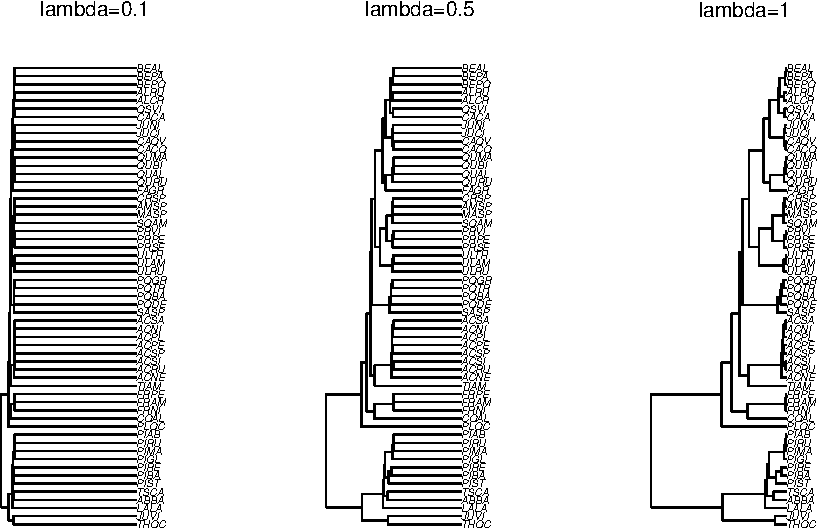
\includegraphics{pcm-workshop_files/figure-latex/alpha example-1} \end{center}

Vous pouvez voir qu'avec des valeurs de lambda faibles, le poids accordé à l'histoire partagée (la phylogénie) est considérablement réduit. Les longues branches terminales indiquent en quelque sorte qu'il pourrait y avoir beaucoup plus de variation dans les résidus indépendants des autres espèces. Cette variation pourrait être due à d'autres facteurs inclus dans les estimations de chaque espèce mais indépendants de la phylogénie (comme les erreurs de mesure, par exemple).

\section{Exercices pratiques}\label{exercices-pratiques-1}

Le modèle \(\lambda\) de Pagel peut être utilisé dans les PGLS en utilisant la structure de corrélation \texttt{corPagel}. L'utilisation de cette structure de corrélation est similaire à celle de la structure \texttt{corBrownian}, sauf que vous devez fournir une valeur de paramètre initiale pour \(\lambda\).

\begin{Shaded}
\begin{Highlighting}[]
\CommentTok{\# Obtenir la structure de corrélation}
\NormalTok{pagel.corr }\OtherTok{\textless{}{-}} \FunctionTok{corPagel}\NormalTok{(}\FloatTok{0.3}\NormalTok{, }\AttributeTok{phy=}\NormalTok{seedplantstree, }\AttributeTok{fixed=}\ConstantTok{FALSE}\NormalTok{, }\AttributeTok{form=}\SpecialCharTok{\textasciitilde{}}\NormalTok{Code)}
\end{Highlighting}
\end{Shaded}

La valeur donnée à corPagel est la valeur de départ pour le paramètre \(\lambda\). Notez également que l'option \texttt{fixed=} est définie sur \texttt{FALSE}. Cela signifie que le paramètre \(\lambda\) sera optimisé en utilisant les moindres carrés généralisés. S'il était défini sur \texttt{TRUE}, alors le modèle serait ajusté avec le paramètre de départ, ici \texttt{0.3}. Le terme \texttt{form\textasciitilde{}Code} indique à la fonction d'utiliser l'ordre de la variable \texttt{Code} pour ordonner les noms d'espèces dans l'arbre.

Ajustons maintenant le PGLS avec cette structure de corrélation.

\begin{Shaded}
\begin{Highlighting}[]
\CommentTok{\# PGLS avec corPagel}
\NormalTok{shade.pgls2 }\OtherTok{\textless{}{-}} \FunctionTok{gls}\NormalTok{(Shade }\SpecialCharTok{\textasciitilde{}}\NormalTok{ Wd, }\AttributeTok{data =}\NormalTok{ seedplantsdata, }\AttributeTok{correlation=}\NormalTok{pagel.corr)}
\FunctionTok{summary}\NormalTok{(shade.pgls2)}
\end{Highlighting}
\end{Shaded}

\begin{verbatim}
## Generalized least squares fit by REML
##   Model: Shade ~ Wd 
##   Data: seedplantsdata 
##        AIC     BIC    logLik
##   163.3967 171.426 -77.69833
## 
## Correlation Structure: corPagel
##  Formula: ~Code 
##  Parameter estimate(s):
##    lambda 
## 0.9581665 
## 
## Coefficients:
##                Value Std.Error   t-value p-value
## (Intercept) 1.254987  1.636575 0.7668377  0.4465
## Wd          3.573527  1.497808 2.3858381  0.0205
## 
##  Correlation: 
##    (Intr)
## Wd -0.397
## 
## Standardized residuals:
##         Min          Q1         Med          Q3         Max 
## -0.75145692 -0.44908843 -0.05417524  0.25655008  0.96493685 
## 
## Residual standard error: 2.621947 
## Degrees of freedom: 57 total; 55 residual
\end{verbatim}

Vous pouvez voir que gls a estimé le paramètre \(\lambda\), qui est ici de 0,958. Étant donné que le \(\lambda\) estimé est très proche de 1, nous pouvons conclure que les résidus du modèle étaient fortement corrélés phylogénétiquement. Cela confirme donc l'importance d'utiliser un PGLS avec ce modèle. Si le \(\lambda\) estimé avait été proche de 0, cela aurait suggéré que le PGLS n'était pas nécessaire. Notez cependant qu'en utilisant cette approche, vous êtes assuré de ne jamais obtenir un résultat statistiquement biaisé. En fait, je vous \textbf{recommande fortement} d'utiliser toujours cette structure de corrélation dans vos analyses statistiques.

\section{Défi no. 4}\label{duxe9fi-no.-4}

Essayez d'ajuster un PGLS avec une structure de corrélation de Pagel en régressant la tolérance à l'ombre sur la masse des graines. Les résidus sont-ils aussi corrélés phylogénétiquement que dans la régression précédente avec la densité du bois?

\section{Autres structures de corrélation (ou modèles évolutifs)}\label{autres-structures-de-corruxe9lation-ou-moduxe8les-uxe9volutifs}

Les structures de corrélation disponibles dans le package \texttt{ape} offrent d'autres alternatives pour le modèle d'évolution des caractères supposé. Par exemple, la structure de corrélation \texttt{corMartins} modélise la sélection en utilisant le modèle d'Ornstein-Uhlenbeck (ou Hansen) avec le paramètre \(\alpha\) qui détermine la force de la sélection. De plus, \texttt{corBlomberg} modélise une évolution brownienne accélérée ou décélérée, c'est-à-dire que le taux d'évolution du mouvement brownien s'accélère ou ralentit avec le temps avec ce modèle. Il est possible de faire des comparaisons de modèles pour décider quel modèle correspond le mieux à la variation résiduelle.

\chapter{ANOVA phylogénétique}\label{anova-phyloguxe9nuxe9tique}

Jusqu'à présent, nous n'avons analysé que des caractères quantitatifs continus. Mais il est également possible de réaliser une ANOVA avec PGLS.

L'avantage de PGLS, tel qu'il est implémenté avec la fonction \texttt{gls}, est qu'il peut être facilement adapté pour tester de nombreux types de modèles différents. Pour donner un exemple ici, il est facile de mettre en œuvre une ANOVA phylogénétique en R. En effet, il vous suffit de fournir à \texttt{gls} un trait catégoriel en tant que variable indépendante.

Comme il n'y a pas de variable catégorielle dans le jeu de données des traits fonctionnels des plantes, nous allons en créer une en divisant la catégorie de densité du bois en deux catégories : bois léger et bois dense.

\begin{Shaded}
\begin{Highlighting}[]
\CommentTok{\# Créer une variable catégorielle}
\NormalTok{seedplantsdata}\SpecialCharTok{$}\NormalTok{Wd.cat}\OtherTok{\textless{}{-}}\FunctionTok{cut}\NormalTok{(seedplantsdata}\SpecialCharTok{$}\NormalTok{Wd,}\AttributeTok{breaks=}\DecValTok{2}\NormalTok{,}\AttributeTok{labels=}\FunctionTok{c}\NormalTok{(}\StringTok{"light"}\NormalTok{,}\StringTok{"dense"}\NormalTok{))}
\CommentTok{\# Regarder le résultat}
\NormalTok{seedplantsdata}\SpecialCharTok{$}\NormalTok{Wd.cat}
\end{Highlighting}
\end{Shaded}

\begin{verbatim}
##  [1] light light dense light dense dense dense light light light light dense
## [13] dense light light dense dense dense dense dense dense dense light dense
## [25] light dense light light dense dense light light light light light light
## [37] light light light light light light light light light dense dense dense
## [49] dense light light light light light light light dense
## Levels: light dense
\end{verbatim}

Nous pouvons maintenant ajuster une ANOVA phylogénétique.

\begin{Shaded}
\begin{Highlighting}[]
\CommentTok{\# ANOVA phylogénétique}
\NormalTok{shade.pgls3 }\OtherTok{\textless{}{-}} \FunctionTok{gls}\NormalTok{(Shade }\SpecialCharTok{\textasciitilde{}}\NormalTok{ Wd.cat, }\AttributeTok{data =}\NormalTok{ seedplantsdata, }\AttributeTok{correlation=}\NormalTok{pagel.corr)}
\FunctionTok{summary}\NormalTok{(shade.pgls3)}
\end{Highlighting}
\end{Shaded}

\begin{verbatim}
## Generalized least squares fit by REML
##   Model: Shade ~ Wd.cat 
##   Data: seedplantsdata 
##        AIC      BIC    logLik
##   166.7352 174.7646 -79.36762
## 
## Correlation Structure: corPagel
##  Formula: ~Code 
##  Parameter estimate(s):
##    lambda 
## 0.9439646 
## 
## Coefficients:
##                 Value Std.Error  t-value p-value
## (Intercept) 2.6826723 1.3844404 1.937730  0.0578
## Wd.catdense 0.6179855 0.2526902 2.445626  0.0177
## 
##  Correlation: 
##             (Intr)
## Wd.catdense -0.037
## 
## Standardized residuals:
##         Min          Q1         Med          Q3         Max 
## -0.69257567 -0.48677930 -0.04143001  0.33640615  0.95379525 
## 
## Residual standard error: 2.429586 
## Degrees of freedom: 57 total; 55 residual
\end{verbatim}

Vous pouvez voir que la densité du bois, même transformée en variable catégorielle, a un effet significatif sur la tolérance à l'ombre.

\chapter{Comparaison de modèles}\label{comparaison-de-moduxe8les}

Vous pourriez être intéressé à comparer différents modèles, ce qui est une approche courante en biologie pour la modélisation. Cependant, il y a une petite subtilité à prendre en compte avec les PGLS.

La méthode par défaut pour l'ajustement des modèles avec \texttt{gls} est l'estimation par maximum de vraisemblance restreinte (REML), obtenue avec \texttt{method="REML"}. Cela diffère de l'estimation standard par maximum de vraisemblance (ML), qui peut être obtenue avec \texttt{method="ML"}. La différence entre ces deux méthodes est complexe, mais il suffit de dire qu'elles diffèrent dans la manière dont les paramètres de variance sont estimés. REML fournit des estimations de paramètres moins biaisées et est la méthode privilégiée pour rapporter les coefficients des paramètres dans une publication. C'est également la méthode de choix si vous souhaitez comparer des modèles avec des structures de corrélation (ou de variance) différentes \citep{zuur2009mixed}. Par exemple, si vous voulez tester si un modèle PGLS avec un \(\lambda\) de Pagel optimisé s'ajuste mieux aux données qu'un modèle sans corrélation phylogénétique (c'est-à-dire avec \(\lambda\) de Pagel = 0) :

\begin{Shaded}
\begin{Highlighting}[]
\NormalTok{pagel}\FloatTok{.0} \OtherTok{\textless{}{-}} \FunctionTok{gls}\NormalTok{(Shade }\SpecialCharTok{\textasciitilde{}}\NormalTok{ Wd, }\AttributeTok{data =}\NormalTok{ seedplantsdata, }
               \AttributeTok{correlation=}\FunctionTok{corPagel}\NormalTok{(}\DecValTok{0}\NormalTok{,}\AttributeTok{phy=}\NormalTok{seedplantstree, }
                                    \AttributeTok{fixed=}\ConstantTok{TRUE}\NormalTok{, }\AttributeTok{form=}\SpecialCharTok{\textasciitilde{}}\NormalTok{Code), }
               \AttributeTok{method=}\StringTok{"REML"}\NormalTok{)}
\NormalTok{pagel.fit }\OtherTok{\textless{}{-}} \FunctionTok{gls}\NormalTok{(Shade }\SpecialCharTok{\textasciitilde{}}\NormalTok{ Wd, }\AttributeTok{data =}\NormalTok{ seedplantsdata, }
                 \AttributeTok{correlation=}\FunctionTok{corPagel}\NormalTok{(}\FloatTok{0.8}\NormalTok{,}\AttributeTok{phy=}\NormalTok{seedplantstree, }
                                      \AttributeTok{fixed=}\ConstantTok{FALSE}\NormalTok{, }\AttributeTok{form=}\SpecialCharTok{\textasciitilde{}}\NormalTok{Code),}
                 \AttributeTok{method=}\StringTok{"REML"}\NormalTok{)}
\FunctionTok{anova}\NormalTok{(pagel}\FloatTok{.0}\NormalTok{,pagel.fit)}
\end{Highlighting}
\end{Shaded}

\begin{verbatim}
##           Model df      AIC     BIC    logLik   Test  L.Ratio p-value
## pagel.0       1  3 180.4720 186.494 -87.23602                        
## pagel.fit     2  4 163.3967 171.426 -77.69833 1 vs 2 19.07537  <.0001
\end{verbatim}

Vous pouvez utiliser l'AIC ou le BIC pour comparer le modèle, ou le test du rapport de vraisemblance. Vous pouvez voir ici que le modèle PGLS avec un \(\lambda\) de Pagel ajusté offre un meilleur ajustement que celui avec un \(\lambda=0\) (AIC plus faible). D'ailleurs, il s'agit également d'un test pour déterminer si un modèle PGLS est meilleur qu'un modèle de régression standard, car une structure \texttt{corPagel} avec \(\lambda=0\) est un modèle standard (= pas de corrélation phylogénétique).

Maintenant, si vous êtes intéressé par le test des paramètres fixes dans le modèle, vous devez utiliser l'ajustement par maximum de vraisemblance \citep{zuur2009mixed}. Par exemple, si vous souhaitez utiliser un test du rapport de vraisemblance pour tester le modèle avec la densité du bois comme variable indépendante par rapport à un modèle nul avec seulement l'ordonnée à l'origine, vous pouvez procéder comme suit.

\begin{Shaded}
\begin{Highlighting}[]
\NormalTok{wd }\OtherTok{\textless{}{-}} \FunctionTok{gls}\NormalTok{(Shade }\SpecialCharTok{\textasciitilde{}}\NormalTok{ Wd, }\AttributeTok{data =}\NormalTok{ seedplantsdata,}
          \AttributeTok{correlation=}\FunctionTok{corBrownian}\NormalTok{(}\AttributeTok{phy=}\NormalTok{seedplantstree, }\AttributeTok{form=}\SpecialCharTok{\textasciitilde{}}\NormalTok{Code), }
          \AttributeTok{method=}\StringTok{"ML"}\NormalTok{)}
\NormalTok{null }\OtherTok{\textless{}{-}} \FunctionTok{gls}\NormalTok{(Shade }\SpecialCharTok{\textasciitilde{}} \DecValTok{1}\NormalTok{, }\AttributeTok{data =}\NormalTok{ seedplantsdata,}
            \AttributeTok{correlation=}\FunctionTok{corBrownian}\NormalTok{(}\AttributeTok{phy=}\NormalTok{seedplantstree, }\AttributeTok{form=}\SpecialCharTok{\textasciitilde{}}\NormalTok{Code), }
            \AttributeTok{method=}\StringTok{"ML"}\NormalTok{)}
\FunctionTok{anova}\NormalTok{(wd,null)}
\end{Highlighting}
\end{Shaded}

\begin{verbatim}
##      Model df      AIC      BIC    logLik   Test  L.Ratio p-value
## wd       1  3 222.0088 228.1380 -108.0044                        
## null     2  2 226.4988 230.5848 -111.2494 1 vs 2 6.489907  0.0108
\end{verbatim}

Vous pouvez voir que le modèle avec la variable de densité du bois est meilleur que le modèle avec seulement l'ordonnée à l'origine. Cependant, comme mentionné ci-dessus, étant donné que l'ajustement REML fournit de meilleures estimations des paramètres, vous devrez réajuster le modèle en utilisant REML pour présenter les résultats.

\begin{Shaded}
\begin{Highlighting}[]
\NormalTok{wd.final }\OtherTok{\textless{}{-}} \FunctionTok{gls}\NormalTok{(Shade }\SpecialCharTok{\textasciitilde{}}\NormalTok{ Wd, }\AttributeTok{data =}\NormalTok{ seedplantsdata,}
                \AttributeTok{correlation=}\FunctionTok{corBrownian}\NormalTok{(}\AttributeTok{phy=}\NormalTok{seedplantstree, }\AttributeTok{form=}\SpecialCharTok{\textasciitilde{}}\NormalTok{Code), }
                \AttributeTok{method=}\StringTok{"REML"}\NormalTok{)}
\FunctionTok{summary}\NormalTok{(wd.final)}
\end{Highlighting}
\end{Shaded}

\begin{verbatim}
## Generalized least squares fit by REML
##   Model: Shade ~ Wd 
##   Data: seedplantsdata 
##        AIC      BIC    logLik
##   214.3762 220.3982 -104.1881
## 
## Correlation Structure: corBrownian
##  Formula: ~Code 
##  Parameter estimate(s):
## numeric(0)
## 
## Coefficients:
##                Value Std.Error   t-value p-value
## (Intercept) 0.911433  4.409058 0.2067184  0.8370
## Wd          4.361028  1.693349 2.5753865  0.0127
## 
##  Correlation: 
##    (Intr)
## Wd -0.166
## 
## Standardized residuals:
##         Min          Q1         Med          Q3         Max 
## -0.26890642 -0.16431866 -0.02645422  0.09638984  0.34953444 
## 
## Residual standard error: 7.455109 
## Degrees of freedom: 57 total; 55 residual
\end{verbatim}

\chapter{Quand devrions-nous utiliser les méthodes comparatives~?}\label{quand-devrions-nous-utiliser-les-muxe9thodes-comparatives}

Les méthodes comparatives devraient toujours être utilisées lorsqu'on travaille avec des ensembles de données qui comprennent plusieurs espèces. Un bon conseil est d'utiliser une méthode permettant aux résidus du modèle de ne pas être tous corrélés phylogénétiquement, comme lors de l'utilisation des PGLS avec la structure \texttt{corPagel} ou en utilisant le modèle mixte phylogénétique. Des études antérieures ont montré que l'utilisation de telles méthodes comparatives donne lieu à des estimations plus précises et exactes de l'effet fixe, un taux d'erreur de type I plus faible et une puissance statistique plus grande \citep{revell2010phylogenetic}. Par conséquent, il est toujours avantageux d'utiliser ces méthodes.

Une erreur courante consiste à utiliser les PGLS pour tester le signal phylogénétique dans \(Y\) ou \(X\) en utilisant soit le \(\lambda\) de Pagel ou le \(K\) de Blomberg, et si un signal phylogénétique est présent, utiliser un PGLS pour analyser les données et sinon utiliser une régression standard. C'est une \textbf{grosse erreur}. Comme nous l'avons vu précédemment, les PGLS corrigent la corrélation phylogénétique dans les résidus et non dans les variables. Par conséquent, la présence d'un signal phylogénétique dans les variables ne signifie pas nécessairement que les résidus sont corrélés phylogénétiquement. Et l'inverse est également vrai : les variables peuvent ne pas être corrélées phylogénétiquement, mais les résidus pourraient l'être !

Une autre idée fausse courante concernant les méthodes comparatives est qu'elles éliminent toute variation dans les données liée à la phylogénie et que cela pourrait affecter l'interprétation de la variable d'intérêt. Cela était vrai pour les anciennes méthodes telles que l'autorégression phylogénétique qui, d'abord, éliminait le signal phylogénétique des données avant de les analyser. Ces approches posaient effectivement problème. Mais les méthodes présentées ici ne souffrent pas de ces problèmes. Elles tiennent compte de la structure phylogénétique et la quantifient, mais elles n'éliminent pas la variation du modèle.

\chapter{Un dernier mot~: le problème de la réplication}\label{un-dernier-mot-le-probluxe8me-de-la-ruxe9plication}

Tout biologiste est bien conscient de l'importance de répliquer ses expériences afin d'avoir confiance en ses conclusions. Cela est beaucoup plus complexe lorsque nous considérons l'évolution. Pour tester nos hypothèses sur l'évolution, l'approche idéale serait de rembobiner la ``bande de l'évolution'' (S. J. Gould) et de laisser l'histoire se répéter plusieurs fois pour voir ce qui se passe. Cela n'est malheureusement pas possible, bien que certaines études d'évolution expérimentale parviennent à reproduire des expériences évolutives.

La méthode comparative phylogénétique introduite dans ce tutoriel est une approche appropriée pour nous protéger d'arriver à des conclusions qui ne sont pas fortement soutenues dans un contexte évolutif. Cependant, même cette approche peut parfois échouer. C'est pourquoi une attention supplémentaire est nécessaire dans de telles études.

En interprétant leurs résultats, les biologistes devraient d'abord se demander s'ils ont suffisamment de réplicats dans leurs données pour tirer des conclusions solides. Et par réplicat, j'entends réplicat évolutif. Considérons l'exemple des plantes à graines présenté ci-dessus.

\begin{center}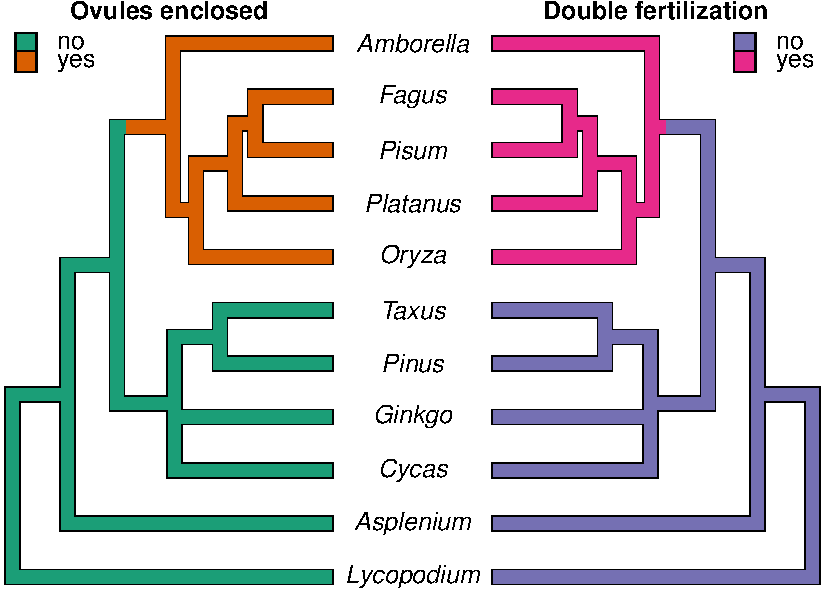
\includegraphics{pcm-workshop_files/figure-latex/AngiospermsWithCharacters4-1} \end{center}

S'il existe plusieurs espèces avec des ovules enfermés ou non et qui effectuent ou non une double fécondation, le scénario le plus parcimonieux pour les deux caractères est que chacun a évolué une fois le long de la branche de l'arbre qui mène aux plantes à fleurs. En d'autres termes, il n'y a eu qu'une seule transition entre les états de chaque caractère dans l'évolution de ce groupe.

Ainsi, même s'il semble y avoir une réplication lorsque nous regardons les espèces (plusieurs espèces avec chaque état de caractère ont été échantillonnées), il n'y a pas de réplication évolutive~! Donc, même si la probabilité que ces deux événements se produisent sur la même branche est très faible et même si un test de contingence pour calculer la probabilité d'un tel événement est significatif, c'est un peu comme une expérience avec un seul réplicat. Par conséquent, même lorsqu'un test qui prend en compte la phylogénie est significatif, une grande prudence est nécessaire lors de l'interprétation de ces résultats. Idéalement, une étude devrait avoir un nombre décent de réplicats évolutifs pour que les résultats soient significatifs sur le plan biologique. Je vous encourage à lire le très bon article de Maddison et Fitzjohn sur le sujet \citep{maddison2015unsolved}.

Idéalement, avant de planifier une expérience, on devrait s'assurer qu'il existe une réplication suffisante dans l'évolution des traits étudiés parmi les espèces considérées pour avoir plus de confiance dans les résultats. Par exemple, il serait beaucoup mieux si chaque caractère avait évolué 5 à 6 fois chacun dans l'exemple précédent, en particulier si les deux caractères évoluaient toujours simultanément~!

\chapter{Le modèle de Mouvement Brownien (BM)}\label{BM-model}

Lorsque nous souhaitons prendre en compte la non-indépendance des espèces en raison de leurs histoires évolutives dans les analyses statistiques, un modèle d'évolution est nécessairement impliqué. En effet, nous supposons que les caractères ont évolué au fil du temps (le long de la phylogénie) et que les espèces étroitement apparentées sont plus susceptibles d'être en moyenne plus similaires pour un trait donné que des espèces éloignées. En biologie évolutive, le modèle de base (souvent utilisé comme modèle nul dans de nombreuses analyses) est le modèle de mouvement brownien. Ce modèle d'évolution porte le nom de Robert Brown, un botaniste célèbre qui a publié une importante \emph{Flora of Australia} en 1810. Il fut aussi le premier à distinguer les gymnospermes des angiospermes. Sa découverte du mouvement brownien est due à l'observation que de petites particules en solution ont tendance à se déplacer dans toutes les directions, une observation faite pour la première fois en observant du pollen de \emph{Clarkia} au microscope. L'explication viendrait plus tard, en termes d'impacts moléculaires aléatoires.

Les mathématiciens ont construit un processus stochastique destiné à approcher le mouvement brownien. Dans ce modèle, chaque étape est indépendante des autres et peut aller dans n'importe quelle direction. Le déplacement moyen est nul et la variance est uniforme dans tout l'espace paramétrique. Les déplacements peuvent être additionnés, ce qui signifie que les variances des déplacements indépendants peuvent s'ajouter. Si \(\sigma^2\) est la variance d'un seul déplacement, la variance après un temps \(t\) sera \(\sigma^2t\). Lorsque le nombre d'étapes est grand, comme dans un contexte phylogénétique, le résultat est distribué normalement.

Lorsqu'il est appliqué aux phylogénies, le modèle de mouvement brownien est en quelque sorte appliqué indépendamment à chaque branche de la phylogénie. Cela permet de modéliser la quantité de changement qui s'est produite le long d'une branche donnée. Si la variance du modèle de mouvement brownien est \(\sigma^2\) par unité de temps \(t\), alors le changement net le long d'une branche de temps \(t\) est tiré d'une distribution normale de moyenne \(0\) et de variance \(\sigma^2t\). Ce modèle peut également être représenté mathématiquement de la manière suivante, où la quantité de changement pour le caractère \(X\) sur le temps infinitésimal dans l'intervalle entre le temps \(t\) et \(t+dt\) est~:

\[dX(t)=\sigma^2 dB(t),\]

où \(dB(t)\) est la distribution gaussienne. Il est important de noter que ce modèle suppose que~:

\begin{enumerate}
\def\labelenumi{\arabic{enumi}.}
\tightlist
\item
  L'évolution se produisant dans chaque branche de la phylogénie est indépendante de celle se produisant dans les autres branches.
\item
  L'évolution est complètement aléatoire (c'est-à-dire sans sélection).
\end{enumerate}

Le paramètre \(\sigma^2\) dans le modèle donne la variance, ou en d'autres termes, la vitesse d'évolution. Plus la variance est élevée, plus le caractère évoluera rapidement. Voici deux exemples de caractères simulés sur un arbre de 200 espèces avec \(\sigma^2=0.5\) et \(\sigma^2=4\).

\begin{center}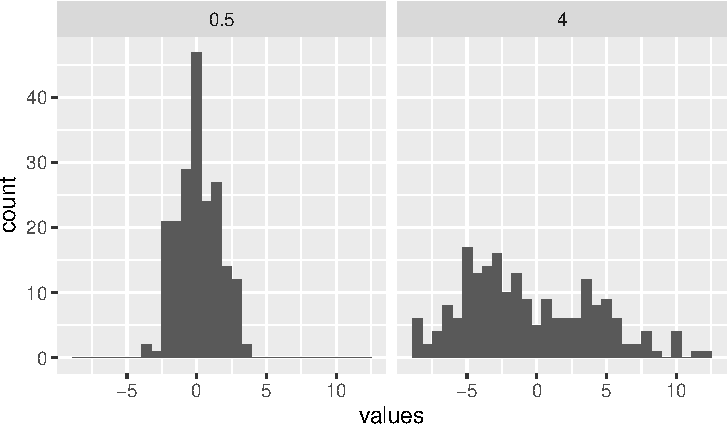
\includegraphics{pcm-workshop_files/figure-latex/BM_Model_SigmaExample-1} \end{center}

Une introduction plus approfondie au modèle de Mouvement Brownien se trouve au chapitre 23 du livre de Joe Felsenstein \citep{felsenstein2004inferring}.

Le modèle de mouvement brownien est souvent dit modéliser la dérive neutre, bien qu'un bon ajustement à ce modèle ne signifie pas nécessairement que les données ont évolué via des dérives aléatoires, car d'autres processus peuvent également donner des motifs similaires à ceux du mouvement brownien \citep{hansen1996translating}.

Notez également que le modèle est stochastique. C'est-à-dire que même si deux espèces étroitement apparentées sont plus susceptibles de partager des états de caractère similaires qu'une espèce éloignée, cela n'est vrai qu'en moyenne. Pour un caractère donné simulé, des espèces étroitement apparentées peuvent parfois être plus différentes qu'une espèce éloignée. Regardez la figure suivante, qui montre trois caractères simulés selon le mouvement brownien.

\begin{center}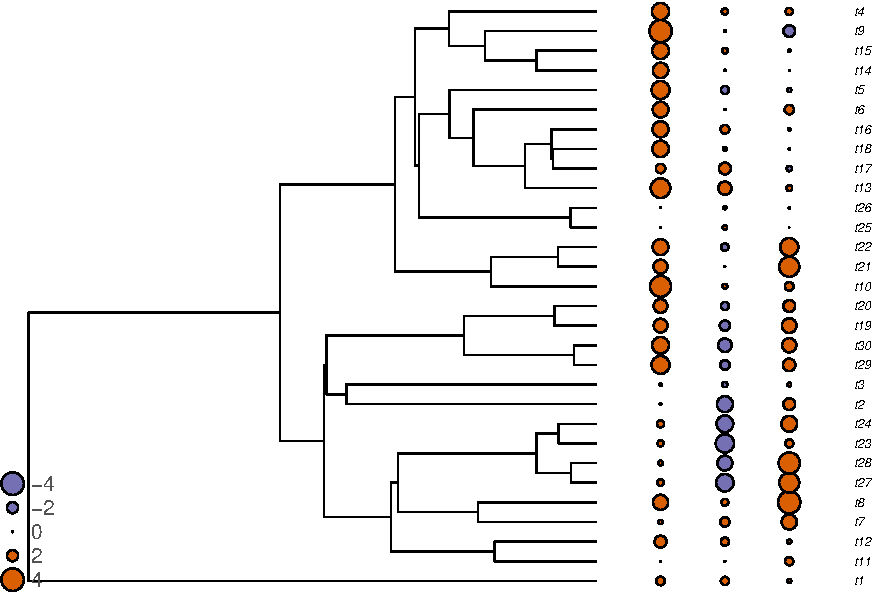
\includegraphics{pcm-workshop_files/figure-latex/PlotContinuousParameter_tablephylo4d-1} \end{center}

\chapter{Lectures supplémentaires}\label{lectures-suppluxe9mentaires}

Pour bien comprendre un nouveau domaine de recherche, il est toujours conseillé de lire beaucoup à ce sujet. Voici quelques références que vous pourriez trouver utiles. Les différentes sources expliquent parfois la théorie de différentes manières ou utilisent des exemples différents, ce qui peut vous aider à mieux comprendre.

\begin{itemize}
\tightlist
\item
  Felsenstein, J. (1985) Phylogenies and the comparative method. \emph{The American Naturalist} 125, 1-15. \textbf{The classic initial paper that launched the field of comparative analyses. The phylogenetic independent contrasts are introduced here}
\item
  Felsenstein, J. (2004) \emph{Inferring phylogenies}. Sinauer Associates, Inc.~Sunderland, MA. \textbf{A thorough reference on phylogenies, from reconstruction to phylogenetic methods}
\item
  Hadfield, J. D., S. Nakagawa. 2010. General quantitative genetic methods for comparative biology: phylogenies, taxonomies and multi-trait models for continuous and categorical characters. \emph{Journal of Evolutionary Biology} 23:494--508. \textbf{This paper describes the phylogenetic mixed model and its implementation in MCMCglmm. It is a very important paper}
\item
  Housworth, E.A., E.P. Martins, M. Lynch. 2004. The phylogenetic mixed model. \emph{The American Naturalist} 163:84--96. \textbf{Excellent paper on the Phylogenetic Mixed Model}
\item
  Paradis, E. (2012). \emph{Analysis of phylogenetics and evolution with R}. New York, USA: Springer. \textbf{This is the book that explains the analyses available in the R package APE. It is also a great reference on many phylogenetic analyses, including the comparative method. This is a classic and a must for users of phylogenies in R.}
\item
  Revell, L J. (2010). Phylogenetic signal and linear regression on species data. \emph{Methods in Ecology and Evolution} 1: 319-329. \textbf{A great paper on PGLS. It uses simulations to show when it is important to use PGLS.}
\item
  Villemereuil, P., S. Nakagawa. 2014. General quantitative genetic methods for comparative biology. Pp. 287--303 in L. Z. Garamszegi, ed.~\emph{Modern phylogenetic comparative methods and their application in evolutionary biology}. Springer-Verlag, Berlin, Heidelberg. \textbf{Nice book chapter explaining the phylogenetic mixed model}
\item
  Zuur, A.F., E.N. Ieno, N. Walker, A. A. Saveliev, G.M. Smith. (2009). \emph{Mixed effects models and extensions in ecology with R}. New York, NY: Springer New York. \textbf{This is not a book on phylogenetic methods, but it is a great book on the analysis of ecological data with examples in R. Its chapter 6 and 7 discuss correlation structures and although they are not about phylogenies, they are very instructive on how to deal with them and how to compare models and analyse complex data. It also has tons of information on how to deal with more complex data, along with correlation structure. A very good read!}
\end{itemize}

\chapter{Introduction aux phylogénies dans R}\label{trees}

Il existe de nombreux packages pour les analyses phylogénétiques dans R. Je ne vais pas tous les énumérer ici, mais vous pouvez avoir une bonne idée des options disponibles en consultant la \href{http://cran.r-project.org/web/views/Phylogenetics.html}{vignette phylogénétique de R} maintenue par Brian O'Meara. Elle est principalement orientée vers les méthodes comparatives phylogénétiques, mais c'est un bon point de départ.

Le package le plus basique pour utiliser des arbres dans R est \emph{ape}, qui vous permet de lire et de tracer des arbres.

\section{Importer et tracer des arbres}\label{importer-et-tracer-des-arbres}

\subsection{Simuler un arbre}\label{simuler-un-arbre}

Tout au long de ces exercices, nous utiliserons souvent des arbres simulés, qui sont très utiles à des fins pédagogiques. Les arbres peuvent être simulés en utilisant plusieurs fonctions, mais voici un exemple pour simuler un arbre avec 15 espèces.

\begin{Shaded}
\begin{Highlighting}[]
\FunctionTok{require}\NormalTok{(phytools)}
\NormalTok{tree }\OtherTok{\textless{}{-}} \FunctionTok{pbtree}\NormalTok{(}\AttributeTok{n=}\DecValTok{15}\NormalTok{,}\AttributeTok{nsim=}\DecValTok{1}\NormalTok{)}
\FunctionTok{plot}\NormalTok{(tree)}
\end{Highlighting}
\end{Shaded}

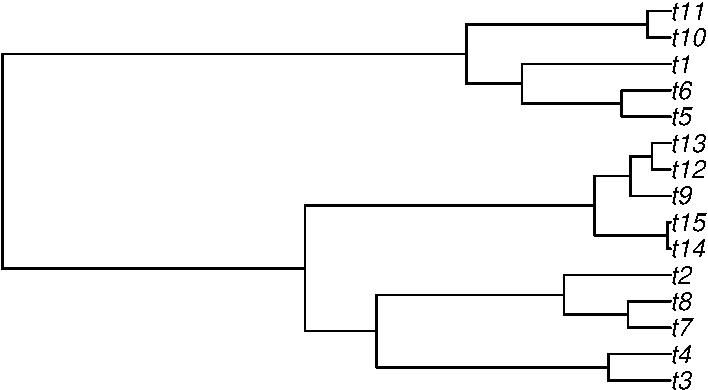
\includegraphics{pcm-workshop_files/figure-latex/Simulate Pure-Birth Tree-1.pdf}

Vous enregistrez l'arbre au format nexus dans un fichier. Mais avant de le faire, il est recommandé de définir le répertoire de travail dans le même dossier où votre script est enregistré. Vous pouvez le faire dans RStudio dans le menu Session\textgreater Set Working Directory\textgreater To Source File Location.

\begin{Shaded}
\begin{Highlighting}[]
\FunctionTok{require}\NormalTok{(ape)}
\FunctionTok{write.nexus}\NormalTok{(tree, }\AttributeTok{file=}\StringTok{"My\_first\_tree.tre"}\NormalTok{)}
\end{Highlighting}
\end{Shaded}

\subsection{Simulation de caractères}\label{simulation-de-caractuxe8res}

Les caractères peuvent également être facilement simulés dans R. Par exemple, vous pourriez simuler un caractère en utilisant un modèle de Mouvement Brownien (BM) avec le code suivant.

\begin{Shaded}
\begin{Highlighting}[]
\NormalTok{trait1 }\OtherTok{\textless{}{-}} \FunctionTok{fastBM}\NormalTok{(tree, }\AttributeTok{sig2=}\FloatTok{0.01}\NormalTok{, }\AttributeTok{nsim=}\DecValTok{1}\NormalTok{, }\AttributeTok{internal=}\ConstantTok{FALSE}\NormalTok{)}
\CommentTok{\# To get trait values for tree tips:}
\NormalTok{trait1}
\end{Highlighting}
\end{Shaded}

\begin{verbatim}
##           t3           t4           t7           t8           t2          t14 
## -0.007306853  0.043251831  0.004858391 -0.114795593 -0.043737891  0.113964926 
##          t15           t9          t12          t13           t5           t6 
##  0.097243984  0.096978766  0.063069656  0.053040643  0.072476832  0.034675083 
##           t1          t10          t11 
## -0.084659118  0.118596501  0.059071786
\end{verbatim}

Ensuite, enregistrons ce trait dans un fichier en faisant comme s'il s'agissait de nos données d'origine.

\begin{Shaded}
\begin{Highlighting}[]
\FunctionTok{write.table}\NormalTok{(}\FunctionTok{matrix}\NormalTok{(trait1,}\AttributeTok{ncol=}\DecValTok{1}\NormalTok{,}\AttributeTok{dimnames=}\FunctionTok{list}\NormalTok{(}\FunctionTok{names}\NormalTok{(trait1),}\StringTok{"trait1"}\NormalTok{)), }\AttributeTok{file=}\StringTok{"mytrait.csv"}\NormalTok{, }\AttributeTok{sep=}\StringTok{";"}\NormalTok{)}
\end{Highlighting}
\end{Shaded}

Maintenant que nous avons simulé un arbre et un caractère, effaçons ce que nous avons fait jusqu'à présent de l'environnement R et faisons comme si c'étaient nos données pour les prochaines sections.

\begin{Shaded}
\begin{Highlighting}[]
\FunctionTok{rm}\NormalTok{(tree, trait1)}
\end{Highlighting}
\end{Shaded}

\section{Importer des données dans R}\label{importer-des-donnuxe9es-dans-r}

Voici comment vous devez importer vos données dans R.

\begin{Shaded}
\begin{Highlighting}[]
\NormalTok{tree }\OtherTok{\textless{}{-}} \FunctionTok{read.nexus}\NormalTok{(}\AttributeTok{file=}\StringTok{"My\_first\_tree.tre"}\NormalTok{)}
\NormalTok{trait1 }\OtherTok{\textless{}{-}} \FunctionTok{read.csv2}\NormalTok{(}\AttributeTok{file=}\StringTok{"mytrait.csv"}\NormalTok{,}\AttributeTok{dec=}\StringTok{"."}\NormalTok{)}
\end{Highlighting}
\end{Shaded}

Le format d'arbre dans ape contient plusieurs informations, et il est utile de savoir comment y accéder. Par exemple, les étiquettes des extrémités peuvent être consultées avec \texttt{tree\$tip.label} et les longueurs des branches avec \texttt{tree\$edge.length}. Nous verrons d'autres options dans d'autres exercices, mais si vous voulez des informations plus détaillées sur la façon dont les objets ``phylo'' sont organisés, vous pouvez consulter le fichier d'aide \texttt{?read.tree} ou ce \href{http://ape-package.ird.fr/misc/FormatTreeR_24Oct2012.pdf}{document} préparé par Emmanuel Paradis, l'auteur de \texttt{ape}.

\section{Représenter des arbres}\label{repruxe9senter-des-arbres}

Tracer des arbres est l'un des aspects les plus intéressants de l'utilisation de R. Les options sont nombreuses et les possibilités larges. La fonction la plus courante est \texttt{plot.phylo} du package ape, qui propose de nombreuses options différentes. Je vous conseille vivement de regarder de près les différentes options de la fonction \texttt{?plot.phylo}. Voici un exemple de base.

\begin{Shaded}
\begin{Highlighting}[]
\FunctionTok{plot}\NormalTok{(tree, }\AttributeTok{type=}\StringTok{"c"}\NormalTok{)}
\FunctionTok{add.scale.bar}\NormalTok{()}
\end{Highlighting}
\end{Shaded}

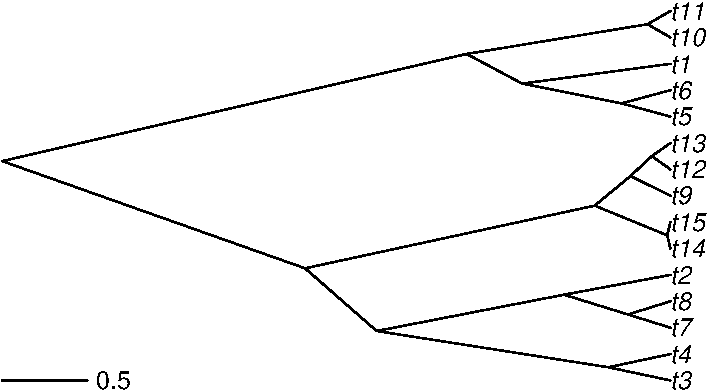
\includegraphics{pcm-workshop_files/figure-latex/Basic tree plotting-1.pdf}

Mais R est aussi intéressant pour représenter des caractères à côté des arbres. Si vous avez un caractère catégoriel, vous pouvez l'utiliser pour colorer les extrémités de la phylogénie.

\begin{Shaded}
\begin{Highlighting}[]
\CommentTok{\# Générer un caractère discret}
\NormalTok{trait2 }\OtherTok{\textless{}{-}} \FunctionTok{as.factor}\NormalTok{(}\FunctionTok{sample}\NormalTok{(}\FunctionTok{c}\NormalTok{(}\DecValTok{1}\NormalTok{,}\DecValTok{2}\NormalTok{,}\DecValTok{3}\NormalTok{),}\AttributeTok{size=}\FunctionTok{length}\NormalTok{(tree}\SpecialCharTok{$}\NormalTok{tip.label),}\AttributeTok{replace=}\ConstantTok{TRUE}\NormalTok{))}
\CommentTok{\# Créer une palette de couleur}
\FunctionTok{library}\NormalTok{(RColorBrewer)}
\NormalTok{ColorPalette1 }\OtherTok{\textless{}{-}} \FunctionTok{brewer.pal}\NormalTok{(}\AttributeTok{n =} \FunctionTok{length}\NormalTok{(}\FunctionTok{levels}\NormalTok{(trait2)), }\AttributeTok{name =} \StringTok{"Dark2"}\NormalTok{)}
\FunctionTok{plot}\NormalTok{(tree, }\AttributeTok{type=}\StringTok{"p"}\NormalTok{, }\AttributeTok{use.edge.length =} \ConstantTok{TRUE}\NormalTok{, }\AttributeTok{label.offset=}\FloatTok{0.2}\NormalTok{,}\AttributeTok{cex=}\DecValTok{1}\NormalTok{)}
\FunctionTok{tiplabels}\NormalTok{(}\AttributeTok{pch=}\DecValTok{21}\NormalTok{,}\AttributeTok{bg=}\NormalTok{ColorPalette1[trait2],}\AttributeTok{col=}\StringTok{"black"}\NormalTok{,}\AttributeTok{cex=}\DecValTok{1}\NormalTok{,}\AttributeTok{adj=}\FloatTok{0.6}\NormalTok{)}
\NormalTok{op}\OtherTok{\textless{}{-}}\FunctionTok{par}\NormalTok{(}\AttributeTok{xpd=}\ConstantTok{TRUE}\NormalTok{)}
\FunctionTok{legend}\NormalTok{(}\DecValTok{0}\NormalTok{,}\DecValTok{0}\NormalTok{,}\AttributeTok{legend=}\FunctionTok{levels}\NormalTok{(trait2),}\AttributeTok{col=}\NormalTok{ColorPalette1,}
       \AttributeTok{pch=}\DecValTok{20}\NormalTok{,}\AttributeTok{bty=}\StringTok{"n"}\NormalTok{,}\AttributeTok{cex=}\DecValTok{1}\NormalTok{,}\AttributeTok{pt.cex=}\FloatTok{1.5}\NormalTok{,}\AttributeTok{ncol=}\FunctionTok{length}\NormalTok{(}\FunctionTok{levels}\NormalTok{(trait2)))}
\end{Highlighting}
\end{Shaded}

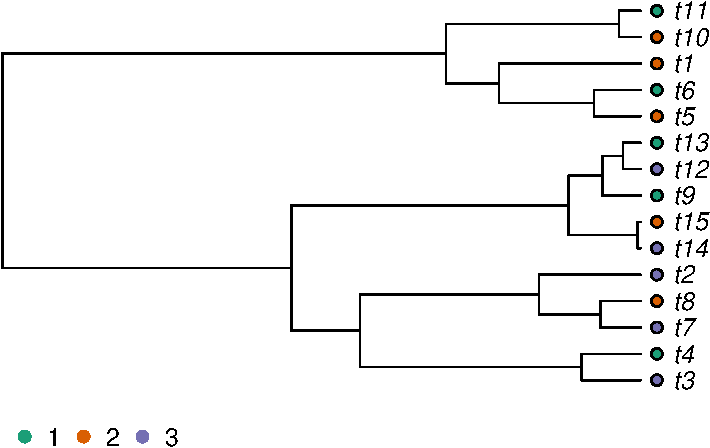
\includegraphics{pcm-workshop_files/figure-latex/Plot categorical parameter-1.pdf}

\begin{Shaded}
\begin{Highlighting}[]
\FunctionTok{par}\NormalTok{(op) }\CommentTok{\#Remettre les paramètres graphiques par défaut}
\end{Highlighting}
\end{Shaded}

Un résultat similaire pourrait être obtenu avec une variable continue. Ici, nous utiliserons le modèle de Mouvement Brownien, que nous étudierons dans une prochaine leçon, pour simuler le caractère continu.

\begin{Shaded}
\begin{Highlighting}[]
\CommentTok{\# Diviser un trait continu en catégories}
\NormalTok{trait1.cat }\OtherTok{\textless{}{-}} \FunctionTok{cut}\NormalTok{(trait1[,}\DecValTok{1}\NormalTok{],}\AttributeTok{breaks=}\DecValTok{8}\NormalTok{,}\AttributeTok{labels=}\ConstantTok{FALSE}\NormalTok{)}
\CommentTok{\# Créer une palette de couleur}
\NormalTok{ColorPalette2 }\OtherTok{\textless{}{-}} \FunctionTok{brewer.pal}\NormalTok{(}\AttributeTok{n =} \DecValTok{8}\NormalTok{, }\AttributeTok{name =} \StringTok{"Blues"}\NormalTok{)}
\CommentTok{\# Représenter l\textquotesingle{}arbre}
\FunctionTok{plot}\NormalTok{(tree, }\AttributeTok{type=}\StringTok{"p"}\NormalTok{, }\AttributeTok{use.edge.length =} \ConstantTok{TRUE}\NormalTok{, }\AttributeTok{label.offset=}\FloatTok{0.2}\NormalTok{,}\AttributeTok{cex=}\DecValTok{1}\NormalTok{)}
\FunctionTok{tiplabels}\NormalTok{(}\AttributeTok{pch=}\DecValTok{21}\NormalTok{,}\AttributeTok{bg=}\NormalTok{ColorPalette2[trait1.cat],}\AttributeTok{col=}\StringTok{"black"}\NormalTok{,}\AttributeTok{cex=}\DecValTok{1}\NormalTok{,}\AttributeTok{adj=}\FloatTok{0.6}\NormalTok{)}
\NormalTok{op}\OtherTok{\textless{}{-}}\FunctionTok{par}\NormalTok{(}\AttributeTok{xpd=}\ConstantTok{TRUE}\NormalTok{)}
\FunctionTok{legend}\NormalTok{(}\DecValTok{0}\NormalTok{,}\DecValTok{0}\NormalTok{,}\AttributeTok{legend=}\FunctionTok{levels}\NormalTok{(}\FunctionTok{cut}\NormalTok{(trait1[,}\DecValTok{1}\NormalTok{],}\AttributeTok{breaks=}\DecValTok{8}\NormalTok{)),}
       \AttributeTok{col=}\NormalTok{ColorPalette2,}\AttributeTok{pch=}\DecValTok{20}\NormalTok{,}\AttributeTok{bty=}\StringTok{"n"}\NormalTok{,}\AttributeTok{cex=}\FloatTok{0.7}\NormalTok{,}\AttributeTok{pt.cex=}\FloatTok{1.5}\NormalTok{,}\AttributeTok{ncol=}\DecValTok{4}\NormalTok{)}
\end{Highlighting}
\end{Shaded}

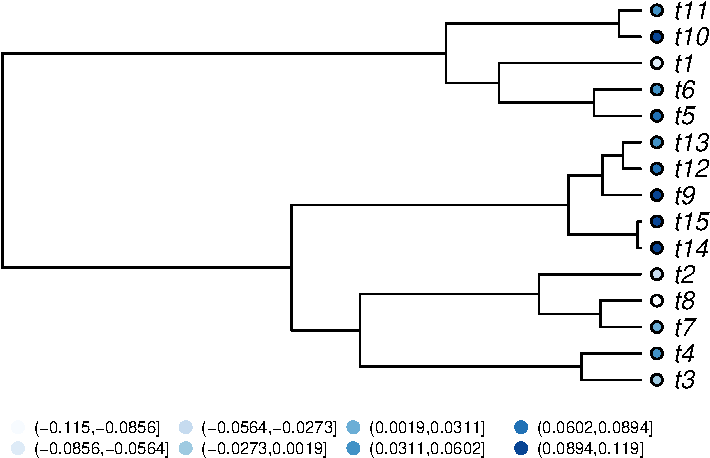
\includegraphics{pcm-workshop_files/figure-latex/Plot continuous parameter-1.pdf}

\begin{Shaded}
\begin{Highlighting}[]
\FunctionTok{par}\NormalTok{(op)}
\end{Highlighting}
\end{Shaded}

Comme prévu pour un caractère simulé avec un mouvement brownien, vous pouvez voir que les espèces étroitement apparentées ont tendance à avoir des valeurs de caractère plus similaires.

Une autre option pour représenter un paramètre continu est d'utiliser la fonction \texttt{table.phylo4d} du package \texttt{adephylo} pour représenter le trait, où ses valeurs sont représentées par des tailles et des couleurs différentes. Il est également possible de tracer plusieurs caractères en même temps.

Notez que vous devrez installer les packages \texttt{phylobase} et \texttt{adephylo} pour exécuter ces fonctions s'ils ne sont pas installés.

\begin{Shaded}
\begin{Highlighting}[]
\FunctionTok{library}\NormalTok{(phylobase)}
\FunctionTok{library}\NormalTok{(adephylo)}
\NormalTok{trait3 }\OtherTok{\textless{}{-}} \FunctionTok{fastBM}\NormalTok{(tree, }\AttributeTok{sig2=}\FloatTok{0.1}\NormalTok{, }\AttributeTok{nsim=}\DecValTok{1}\NormalTok{, }\AttributeTok{internal=}\ConstantTok{FALSE}\NormalTok{) }\CommentTok{\#simuler un caractère}
\NormalTok{trait.table }\OtherTok{\textless{}{-}} \FunctionTok{data.frame}\NormalTok{(}\AttributeTok{trait1=}\NormalTok{trait1[,}\DecValTok{1}\NormalTok{], trait3)}
\NormalTok{obj }\OtherTok{\textless{}{-}} \FunctionTok{phylo4d}\NormalTok{(tree, trait.table) }\CommentTok{\# construire un objet phylo4d}
\NormalTok{op }\OtherTok{\textless{}{-}} \FunctionTok{par}\NormalTok{(}\AttributeTok{mar=}\FunctionTok{c}\NormalTok{(}\DecValTok{1}\NormalTok{,}\DecValTok{1}\NormalTok{,}\DecValTok{1}\NormalTok{,}\DecValTok{1}\NormalTok{))}
\FunctionTok{table.phylo4d}\NormalTok{(obj,}\AttributeTok{cex.label=}\DecValTok{1}\NormalTok{,}\AttributeTok{cex.symbol=}\DecValTok{1}\NormalTok{,}\AttributeTok{ratio.tree=}\FloatTok{0.8}\NormalTok{,}\AttributeTok{grid=}\ConstantTok{FALSE}\NormalTok{,}\AttributeTok{box=}\ConstantTok{FALSE}\NormalTok{)}
\end{Highlighting}
\end{Shaded}

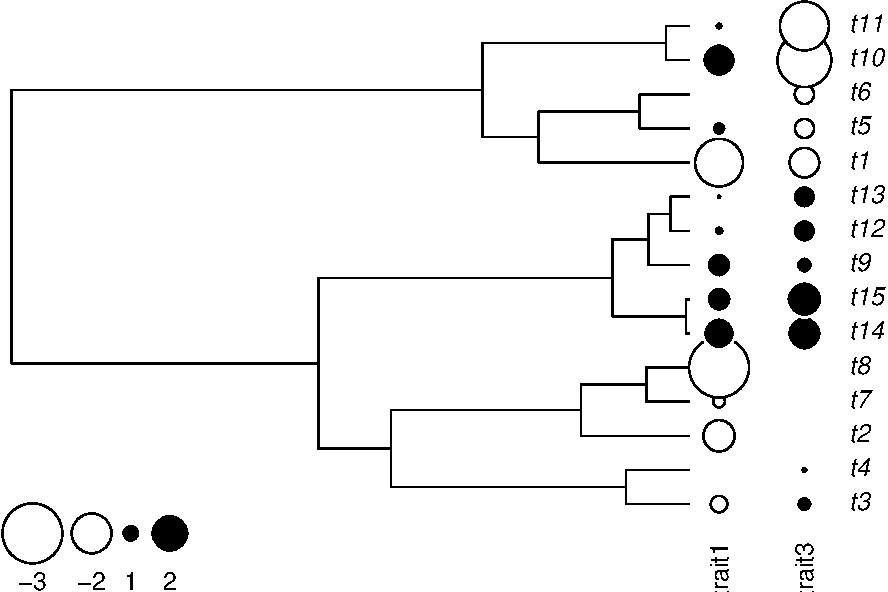
\includegraphics{pcm-workshop_files/figure-latex/Plot continuous parameter - table.phylo4d-1.pdf}

\begin{Shaded}
\begin{Highlighting}[]
\FunctionTok{par}\NormalTok{(op)}
\end{Highlighting}
\end{Shaded}

On peut aussi représenter avec un traitgram:

\begin{Shaded}
\begin{Highlighting}[]
\FunctionTok{require}\NormalTok{(phytools)}
\FunctionTok{phenogram}\NormalTok{(tree,trait3,}\AttributeTok{spread.labels=}\ConstantTok{TRUE}\NormalTok{)}
\end{Highlighting}
\end{Shaded}

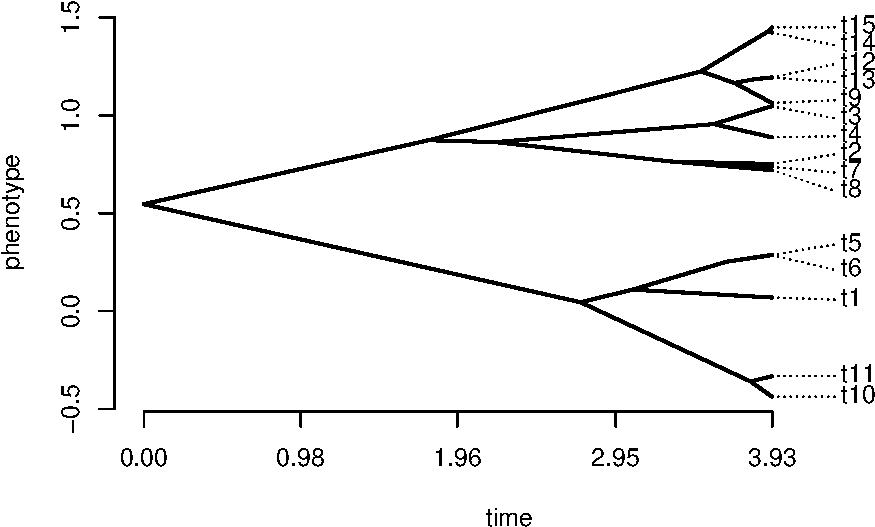
\includegraphics{pcm-workshop_files/figure-latex/traitgram-1.pdf}

Enfin, il est également possible de représenter un arbre sur un graphique en deux dimensions, en colorant les points avec la variable catégorielle.

\begin{Shaded}
\begin{Highlighting}[]
\FunctionTok{phylomorphospace}\NormalTok{(tree,trait.table)}
\FunctionTok{points}\NormalTok{(trait.table,}\AttributeTok{pch=}\DecValTok{21}\NormalTok{,}\AttributeTok{bg=}\NormalTok{ColorPalette1[trait2],}\AttributeTok{col=}\StringTok{"black"}\NormalTok{,}\AttributeTok{cex=}\FloatTok{1.2}\NormalTok{,}\AttributeTok{adj=}\DecValTok{1}\NormalTok{)}
\FunctionTok{legend}\NormalTok{(}\StringTok{"topleft"}\NormalTok{,}\AttributeTok{legend=}\FunctionTok{levels}\NormalTok{(trait2),}
       \AttributeTok{col=}\NormalTok{ColorPalette1,}\AttributeTok{pch=}\DecValTok{20}\NormalTok{,}\AttributeTok{bty=}\StringTok{"n"}\NormalTok{,}\AttributeTok{cex=}\DecValTok{1}\NormalTok{,}\AttributeTok{pt.cex=}\FloatTok{1.5}\NormalTok{,}\AttributeTok{ncol=}\FunctionTok{length}\NormalTok{(}\FunctionTok{levels}\NormalTok{(trait2)))}
\end{Highlighting}
\end{Shaded}

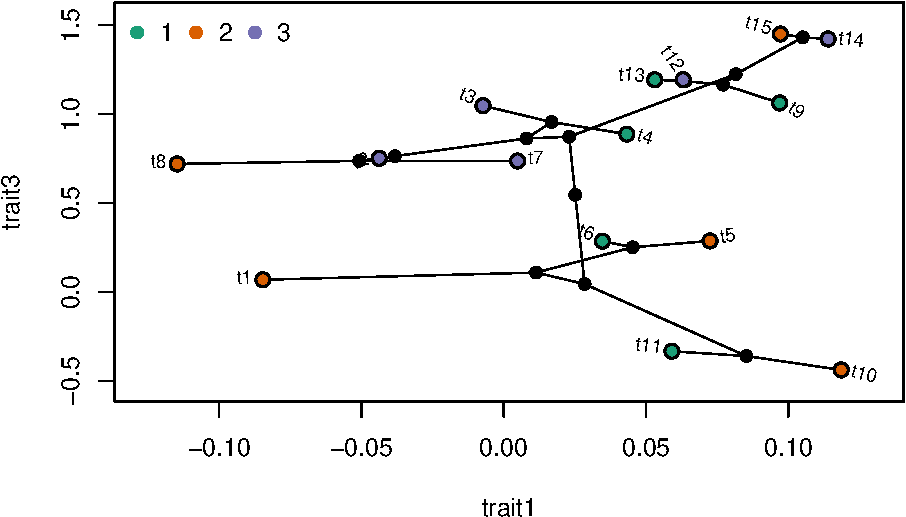
\includegraphics{pcm-workshop_files/figure-latex/Phylomorphospace-1.pdf}

\section{Gérer plusieurs arbres}\label{guxe9rer-plusieurs-arbres}

Dans plusieurs cas, il est important de savoir comment gérer plusieurs arbres dans R. Ceux-ci sont normalement stockés dans un objet \texttt{multiPhylo}. Voyons un exemple.

\begin{Shaded}
\begin{Highlighting}[]
\NormalTok{trees }\OtherTok{\textless{}{-}} \FunctionTok{pbtree}\NormalTok{(}\AttributeTok{n=}\DecValTok{15}\NormalTok{,}\AttributeTok{nsim=}\DecValTok{10}\NormalTok{)}
\NormalTok{trees}
\end{Highlighting}
\end{Shaded}

\begin{verbatim}
## 10 phylogenetic trees
\end{verbatim}

Vous pouvez voir que l'objet n'est pas le même qu'un objet phylo. Par exemple, si vous utilisez le code \texttt{plot(trees)}, vous serez invité à appuyer sur Entrée pour passer d'un arbre à l'autre. Pour accéder aux arbres individuels, vous devez utiliser la technique suivante.

\begin{Shaded}
\begin{Highlighting}[]
\NormalTok{trees[[}\DecValTok{1}\NormalTok{]]}
\end{Highlighting}
\end{Shaded}

\begin{verbatim}
## 
## Phylogenetic tree with 15 tips and 14 internal nodes.
## 
## Tip labels:
##   t3, t4, t5, t14, t15, t8, ...
## 
## Rooted; includes branch lengths.
\end{verbatim}

\begin{Shaded}
\begin{Highlighting}[]
\FunctionTok{plot}\NormalTok{(trees[[}\DecValTok{1}\NormalTok{]])}
\end{Highlighting}
\end{Shaded}

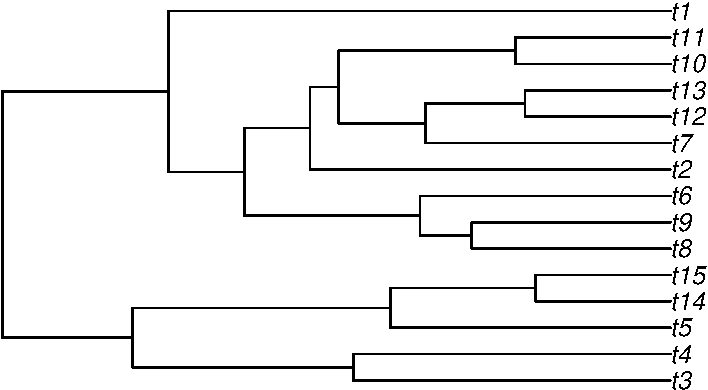
\includegraphics{pcm-workshop_files/figure-latex/multiPhylo manipulation-1.pdf}

\section{Manipuler les arbres}\label{manipuler-les-arbres}

Il existe plusieurs manipulations qui peuvent être effectuées sur les arbres. Voici quelques exemples.

\subsection{Supprimer des feuilles de l'arbre}\label{supprimer-des-feuilles-de-larbre}

\begin{Shaded}
\begin{Highlighting}[]
\FunctionTok{plot}\NormalTok{(}\FunctionTok{drop.tip}\NormalTok{(tree,}\FunctionTok{c}\NormalTok{(}\StringTok{"t1"}\NormalTok{,}\StringTok{"t2"}\NormalTok{,}\StringTok{"t3"}\NormalTok{,}\StringTok{"t4"}\NormalTok{,}\StringTok{"t5"}\NormalTok{)))}
\end{Highlighting}
\end{Shaded}

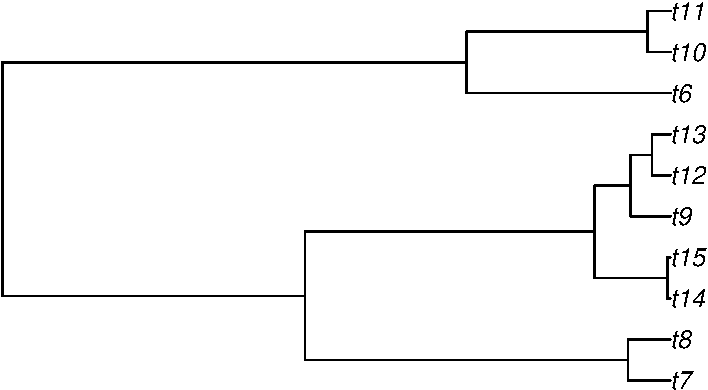
\includegraphics{pcm-workshop_files/figure-latex/Drop tips-1.pdf}

\subsection{Réenraciner les arbres}\label{ruxe9enraciner-les-arbres}

\begin{Shaded}
\begin{Highlighting}[]
\FunctionTok{plot}\NormalTok{(}\FunctionTok{root}\NormalTok{(tree,}\StringTok{"t1"}\NormalTok{))}
\end{Highlighting}
\end{Shaded}

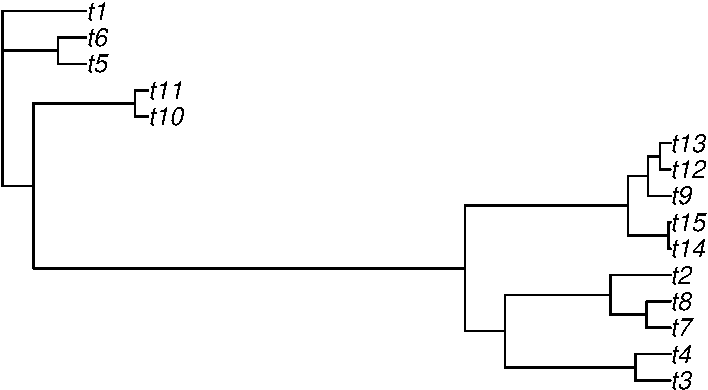
\includegraphics{pcm-workshop_files/figure-latex/Reroot trees-1.pdf}

\subsection{Obtenir les distances cophénétiques}\label{obtenir-les-distances-cophuxe9nuxe9tiques}

\begin{Shaded}
\begin{Highlighting}[]
\FunctionTok{cophenetic.phylo}\NormalTok{(tree)}
\end{Highlighting}
\end{Shaded}

\begin{verbatim}
##            t3        t4        t7        t8       t2        t14        t15
## t3  0.0000000 0.7285289 3.4533793 3.4533793 3.453379 4.29496600 4.29496600
## t4  0.7285289 0.0000000 3.4533793 3.4533793 3.453379 4.29496600 4.29496600
## t7  3.4533793 3.4533793 0.0000000 0.4962115 1.250834 4.29496600 4.29496600
## t8  3.4533793 3.4533793 0.4962115 0.0000000 1.250834 4.29496600 4.29496600
## t2  3.4533793 3.4533793 1.2508336 1.2508336 0.000000 4.29496600 4.29496600
## t14 4.2949660 4.2949660 4.2949660 4.2949660 4.294966 0.00000000 0.03691962
## t15 4.2949660 4.2949660 4.2949660 4.2949660 4.294966 0.03691962 0.00000000
## t9  4.2949660 4.2949660 4.2949660 4.2949660 4.294966 0.88909442 0.88909442
## t12 4.2949660 4.2949660 4.2949660 4.2949660 4.294966 0.88909442 0.88909442
## t13 4.2949660 4.2949660 4.2949660 4.2949660 4.294966 0.88909442 0.88909442
## t5  7.8556290 7.8556290 7.8556290 7.8556290 7.855629 7.85562897 7.85562897
## t6  7.8556290 7.8556290 7.8556290 7.8556290 7.855629 7.85562897 7.85562897
## t1  7.8556290 7.8556290 7.8556290 7.8556290 7.855629 7.85562897 7.85562897
## t10 7.8556290 7.8556290 7.8556290 7.8556290 7.855629 7.85562897 7.85562897
## t11 7.8556290 7.8556290 7.8556290 7.8556290 7.855629 7.85562897 7.85562897
##            t9       t12       t13        t5        t6       t1      t10
## t3  4.2949660 4.2949660 4.2949660 7.8556290 7.8556290 7.855629 7.855629
## t4  4.2949660 4.2949660 4.2949660 7.8556290 7.8556290 7.855629 7.855629
## t7  4.2949660 4.2949660 4.2949660 7.8556290 7.8556290 7.855629 7.855629
## t8  4.2949660 4.2949660 4.2949660 7.8556290 7.8556290 7.855629 7.855629
## t2  4.2949660 4.2949660 4.2949660 7.8556290 7.8556290 7.855629 7.855629
## t14 0.8890944 0.8890944 0.8890944 7.8556290 7.8556290 7.855629 7.855629
## t15 0.8890944 0.8890944 0.8890944 7.8556290 7.8556290 7.855629 7.855629
## t9  0.0000000 0.4685481 0.4685481 7.8556290 7.8556290 7.855629 7.855629
## t12 0.4685481 0.0000000 0.2174902 7.8556290 7.8556290 7.855629 7.855629
## t13 0.4685481 0.2174902 0.0000000 7.8556290 7.8556290 7.855629 7.855629
## t5  7.8556290 7.8556290 7.8556290 0.0000000 0.5720997 1.742611 2.395633
## t6  7.8556290 7.8556290 7.8556290 0.5720997 0.0000000 1.742611 2.395633
## t1  7.8556290 7.8556290 7.8556290 1.7426110 1.7426110 0.000000 2.395633
## t10 7.8556290 7.8556290 7.8556290 2.3956328 2.3956328 2.395633 0.000000
## t11 7.8556290 7.8556290 7.8556290 2.3956328 2.3956328 2.395633 0.268201
##          t11
## t3  7.855629
## t4  7.855629
## t7  7.855629
## t8  7.855629
## t2  7.855629
## t14 7.855629
## t15 7.855629
## t9  7.855629
## t12 7.855629
## t13 7.855629
## t5  2.395633
## t6  2.395633
## t1  2.395633
## t10 0.268201
## t11 0.000000
\end{verbatim}

\chapter{Solutions aux défis}\label{solutions}

\section{Défi 1}\label{duxe9fi-1}

Dans la trame de données \texttt{seedplantsdata}, il y avait de nombreux traits différents. Essayez d'ajuster une régression de la tolérance à l'ombre des arbres (\texttt{Shade}) en fonction de la masse des graines (\texttt{Sm}). En d'autres termes, testez si la tolérance à l'ombre peut être expliquée par la masse des graines des arbres. Ensuite, essayez de voir si les résidus sont corrélés phylogénétiquement.

\begin{Shaded}
\begin{Highlighting}[]
\CommentTok{\# Ajuster un modèle linéaire en utilisant les moindres carrés (Ordinary Least Squares; OLS)}
\NormalTok{Sm.lm }\OtherTok{\textless{}{-}} \FunctionTok{lm}\NormalTok{(Shade }\SpecialCharTok{\textasciitilde{}}\NormalTok{ Sm, }\AttributeTok{data =}\NormalTok{ seedplantsdata)}
\FunctionTok{summary}\NormalTok{(Sm.lm)}
\end{Highlighting}
\end{Shaded}

\begin{verbatim}
## 
## Call:
## lm(formula = Shade ~ Sm, data = seedplantsdata)
## 
## Residuals:
##     Min      1Q  Median      3Q     Max 
## -1.9042 -0.9009  0.1481  0.5982  2.0962 
## 
## Coefficients:
##               Estimate Std. Error t value Pr(>|t|)    
## (Intercept)  2.904e+00  1.608e-01  18.064   <2e-16 ***
## Sm          -5.824e-05  5.640e-05  -1.033    0.306    
## ---
## Signif. codes:  0 '***' 0.001 '**' 0.01 '*' 0.05 '.' 0.1 ' ' 1
## 
## Residual standard error: 1.149 on 55 degrees of freedom
## Multiple R-squared:  0.01902,    Adjusted R-squared:  0.001184 
## F-statistic: 1.066 on 1 and 55 DF,  p-value: 0.3063
\end{verbatim}

\begin{Shaded}
\begin{Highlighting}[]
\CommentTok{\# Extraire les résidus}
\NormalTok{Sm.res }\OtherTok{\textless{}{-}} \FunctionTok{residuals}\NormalTok{(Sm.lm)}
\CommentTok{\# Représenter les résidus à côté de la phylogénie}
\NormalTok{op }\OtherTok{\textless{}{-}} \FunctionTok{par}\NormalTok{(}\AttributeTok{mar=}\FunctionTok{c}\NormalTok{(}\DecValTok{1}\NormalTok{,}\DecValTok{1}\NormalTok{,}\DecValTok{1}\NormalTok{,}\DecValTok{1}\NormalTok{))}
\FunctionTok{plot}\NormalTok{(seedplantstree,}\AttributeTok{type=}\StringTok{"p"}\NormalTok{,}\ConstantTok{TRUE}\NormalTok{,}\AttributeTok{label.offset=}\FloatTok{0.01}\NormalTok{,}\AttributeTok{cex=}\FloatTok{0.5}\NormalTok{,}\AttributeTok{no.margin=}\ConstantTok{FALSE}\NormalTok{)}
\FunctionTok{tiplabels}\NormalTok{(}\AttributeTok{pch=}\DecValTok{21}\NormalTok{,}\AttributeTok{bg=}\NormalTok{cols[}\FunctionTok{ifelse}\NormalTok{(Sm.res}\SpecialCharTok{\textgreater{}}\DecValTok{0}\NormalTok{,}\DecValTok{1}\NormalTok{,}\DecValTok{2}\NormalTok{)],}\AttributeTok{col=}\StringTok{"black"}\NormalTok{,}\AttributeTok{cex=}\FunctionTok{abs}\NormalTok{(Sm.res),}\AttributeTok{adj=}\FloatTok{0.505}\NormalTok{)}
\FunctionTok{legend}\NormalTok{(}\StringTok{"topleft"}\NormalTok{,}\AttributeTok{legend=}\FunctionTok{c}\NormalTok{(}\StringTok{"{-}2"}\NormalTok{,}\StringTok{"{-}1"}\NormalTok{,}\StringTok{"0"}\NormalTok{,}\StringTok{"1"}\NormalTok{,}\StringTok{"2"}\NormalTok{),}\AttributeTok{pch=}\DecValTok{21}\NormalTok{,}
       \AttributeTok{pt.bg=}\NormalTok{cols[}\FunctionTok{c}\NormalTok{(}\DecValTok{1}\NormalTok{,}\DecValTok{1}\NormalTok{,}\DecValTok{1}\NormalTok{,}\DecValTok{2}\NormalTok{,}\DecValTok{2}\NormalTok{)],}\AttributeTok{bty=}\StringTok{"n"}\NormalTok{,}
       \AttributeTok{text.col=}\StringTok{"gray32"}\NormalTok{,}\AttributeTok{cex=}\FloatTok{0.8}\NormalTok{,}\AttributeTok{pt.cex=}\FunctionTok{c}\NormalTok{(}\DecValTok{2}\NormalTok{,}\DecValTok{1}\NormalTok{,}\FloatTok{0.1}\NormalTok{,}\DecValTok{1}\NormalTok{,}\DecValTok{2}\NormalTok{))}
\end{Highlighting}
\end{Shaded}

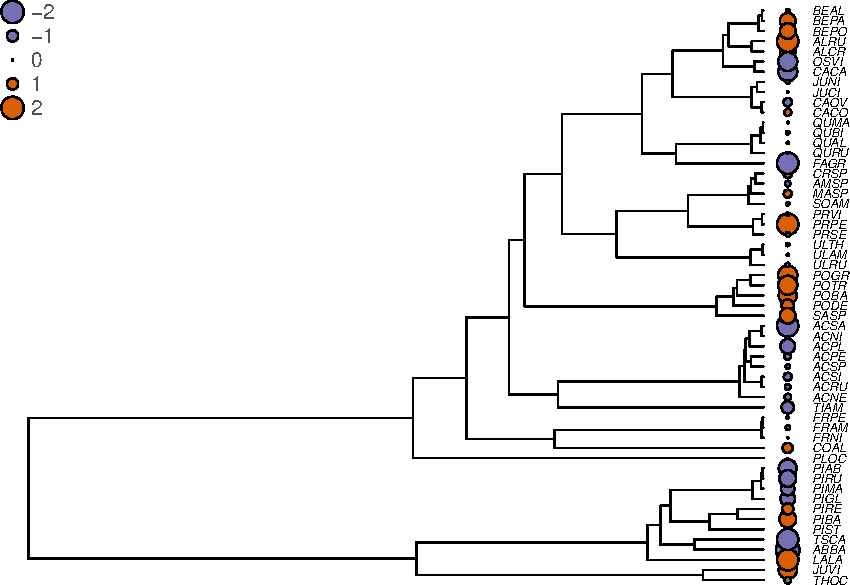
\includegraphics{pcm-workshop_files/figure-latex/Challenge 1 - solution-1.pdf}

\begin{Shaded}
\begin{Highlighting}[]
\FunctionTok{par}\NormalTok{(op)}
\end{Highlighting}
\end{Shaded}

\section{Défi 2}\label{duxe9fi-2}

Pouvez-vous obtenir la matrice de covariance et la matrice de corrélation pour l'arbre phylogénétique des plantes à graines de l'exemple ci-dessus (\texttt{seedplantstree})?

\begin{Shaded}
\begin{Highlighting}[]
\CommentTok{\# Covariance matrix}
\NormalTok{seedplants.cov }\OtherTok{\textless{}{-}} \FunctionTok{vcv}\NormalTok{(seedplantstree,}\AttributeTok{corr=}\ConstantTok{FALSE}\NormalTok{)}
\CommentTok{\# Regarder les premières lignes de la matrice}
\FunctionTok{head}\NormalTok{(}\FunctionTok{round}\NormalTok{(seedplants.cov,}\DecValTok{3}\NormalTok{))}
\end{Highlighting}
\end{Shaded}

\begin{verbatim}
##       ABBA  ACNE  ACNI  ACPE  ACPL  ACRU  ACSA  ACSI  ACSP  ALCR  ALRU  AMSP
## ABBA 0.151 0.000 0.000 0.000 0.000 0.000 0.000 0.000 0.000 0.000 0.000 0.000
## ACNE 0.000 0.151 0.146 0.146 0.146 0.146 0.146 0.146 0.146 0.099 0.099 0.099
## ACNI 0.000 0.146 0.151 0.147 0.148 0.147 0.150 0.147 0.147 0.099 0.099 0.099
## ACPE 0.000 0.146 0.147 0.151 0.147 0.147 0.147 0.147 0.148 0.099 0.099 0.099
## ACPL 0.000 0.146 0.148 0.147 0.151 0.147 0.148 0.147 0.147 0.099 0.099 0.099
## ACRU 0.000 0.146 0.147 0.147 0.147 0.151 0.147 0.150 0.147 0.099 0.099 0.099
##       BEAL  BEPA  BEPO  CACA  CACO  CAOV COAL  CRSP  FAGR FRAM FRNI FRPE  JUCI
## ABBA 0.000 0.000 0.000 0.000 0.000 0.000 0.00 0.000 0.000 0.00 0.00 0.00 0.000
## ACNE 0.099 0.099 0.099 0.099 0.099 0.099 0.09 0.099 0.099 0.09 0.09 0.09 0.099
## ACNI 0.099 0.099 0.099 0.099 0.099 0.099 0.09 0.099 0.099 0.09 0.09 0.09 0.099
## ACPE 0.099 0.099 0.099 0.099 0.099 0.099 0.09 0.099 0.099 0.09 0.09 0.09 0.099
## ACPL 0.099 0.099 0.099 0.099 0.099 0.099 0.09 0.099 0.099 0.09 0.09 0.09 0.099
## ACRU 0.099 0.099 0.099 0.099 0.099 0.099 0.09 0.099 0.099 0.09 0.09 0.09 0.099
##       JUNI JUVI  LALA  MASP  OSVI PIAB PIBA PIGL PIMA PIRE PIRU PIST  PLOC
## ABBA 0.000 0.08 0.127 0.000 0.000 0.13 0.13 0.13 0.13 0.13 0.13 0.13 0.000
## ACNE 0.099 0.00 0.000 0.099 0.099 0.00 0.00 0.00 0.00 0.00 0.00 0.00 0.079
## ACNI 0.099 0.00 0.000 0.099 0.099 0.00 0.00 0.00 0.00 0.00 0.00 0.00 0.079
## ACPE 0.099 0.00 0.000 0.099 0.099 0.00 0.00 0.00 0.00 0.00 0.00 0.00 0.079
## ACPL 0.099 0.00 0.000 0.099 0.099 0.00 0.00 0.00 0.00 0.00 0.00 0.00 0.079
## ACRU 0.099 0.00 0.000 0.099 0.099 0.00 0.00 0.00 0.00 0.00 0.00 0.00 0.079
##       POBA  PODE  POGR  POTR  PRPE  PRSE  PRVI  QUAL  QUBI  QUMA  QURU  SASP
## ABBA 0.000 0.000 0.000 0.000 0.000 0.000 0.000 0.000 0.000 0.000 0.000 0.000
## ACNE 0.099 0.099 0.099 0.099 0.099 0.099 0.099 0.099 0.099 0.099 0.099 0.099
## ACNI 0.099 0.099 0.099 0.099 0.099 0.099 0.099 0.099 0.099 0.099 0.099 0.099
## ACPE 0.099 0.099 0.099 0.099 0.099 0.099 0.099 0.099 0.099 0.099 0.099 0.099
## ACPL 0.099 0.099 0.099 0.099 0.099 0.099 0.099 0.099 0.099 0.099 0.099 0.099
## ACRU 0.099 0.099 0.099 0.099 0.099 0.099 0.099 0.099 0.099 0.099 0.099 0.099
##       SOAM THOC  TIAM  TSCA  ULAM  ULRU  ULTH
## ABBA 0.000 0.08 0.000 0.137 0.000 0.000 0.000
## ACNE 0.099 0.00 0.109 0.000 0.099 0.099 0.099
## ACNI 0.099 0.00 0.109 0.000 0.099 0.099 0.099
## ACPE 0.099 0.00 0.109 0.000 0.099 0.099 0.099
## ACPL 0.099 0.00 0.109 0.000 0.099 0.099 0.099
## ACRU 0.099 0.00 0.109 0.000 0.099 0.099 0.099
\end{verbatim}

\begin{Shaded}
\begin{Highlighting}[]
\CommentTok{\# Matrice de corrélation}
\NormalTok{seedplants.cor }\OtherTok{\textless{}{-}} \FunctionTok{vcv}\NormalTok{(seedplantstree,}\AttributeTok{corr=}\ConstantTok{TRUE}\NormalTok{)}
\CommentTok{\# Regarder les premières lignes de la matrice}
\FunctionTok{head}\NormalTok{(}\FunctionTok{round}\NormalTok{(seedplants.cor,}\DecValTok{3}\NormalTok{))}
\end{Highlighting}
\end{Shaded}

\begin{verbatim}
##      ABBA  ACNE  ACNI  ACPE  ACPL  ACRU  ACSA  ACSI  ACSP  ALCR  ALRU  AMSP
## ABBA    1 0.000 0.000 0.000 0.000 0.000 0.000 0.000 0.000 0.000 0.000 0.000
## ACNE    0 1.000 0.967 0.967 0.967 0.967 0.967 0.967 0.967 0.654 0.654 0.654
## ACNI    0 0.967 1.000 0.976 0.981 0.974 0.997 0.974 0.976 0.654 0.654 0.654
## ACPE    0 0.967 0.976 1.000 0.976 0.974 0.976 0.974 0.983 0.654 0.654 0.654
## ACPL    0 0.967 0.981 0.976 1.000 0.974 0.981 0.974 0.976 0.654 0.654 0.654
## ACRU    0 0.967 0.974 0.974 0.974 1.000 0.974 0.997 0.974 0.654 0.654 0.654
##       BEAL  BEPA  BEPO  CACA  CACO  CAOV  COAL  CRSP  FAGR  FRAM  FRNI  FRPE
## ABBA 0.000 0.000 0.000 0.000 0.000 0.000 0.000 0.000 0.000 0.000 0.000 0.000
## ACNE 0.654 0.654 0.654 0.654 0.654 0.654 0.596 0.654 0.654 0.596 0.596 0.596
## ACNI 0.654 0.654 0.654 0.654 0.654 0.654 0.596 0.654 0.654 0.596 0.596 0.596
## ACPE 0.654 0.654 0.654 0.654 0.654 0.654 0.596 0.654 0.654 0.596 0.596 0.596
## ACPL 0.654 0.654 0.654 0.654 0.654 0.654 0.596 0.654 0.654 0.596 0.596 0.596
## ACRU 0.654 0.654 0.654 0.654 0.654 0.654 0.596 0.654 0.654 0.596 0.596 0.596
##       JUCI  JUNI  JUVI  LALA  MASP  OSVI PIAB PIBA PIGL PIMA PIRE PIRU PIST
## ABBA 0.000 0.000 0.528 0.843 0.000 0.000 0.86 0.86 0.86 0.86 0.86 0.86 0.86
## ACNE 0.654 0.654 0.000 0.000 0.654 0.654 0.00 0.00 0.00 0.00 0.00 0.00 0.00
## ACNI 0.654 0.654 0.000 0.000 0.654 0.654 0.00 0.00 0.00 0.00 0.00 0.00 0.00
## ACPE 0.654 0.654 0.000 0.000 0.654 0.654 0.00 0.00 0.00 0.00 0.00 0.00 0.00
## ACPL 0.654 0.654 0.000 0.000 0.654 0.654 0.00 0.00 0.00 0.00 0.00 0.00 0.00
## ACRU 0.654 0.654 0.000 0.000 0.654 0.654 0.00 0.00 0.00 0.00 0.00 0.00 0.00
##       PLOC  POBA  PODE  POGR  POTR  PRPE  PRSE  PRVI  QUAL  QUBI  QUMA  QURU
## ABBA 0.000 0.000 0.000 0.000 0.000 0.000 0.000 0.000 0.000 0.000 0.000 0.000
## ACNE 0.523 0.654 0.654 0.654 0.654 0.654 0.654 0.654 0.654 0.654 0.654 0.654
## ACNI 0.523 0.654 0.654 0.654 0.654 0.654 0.654 0.654 0.654 0.654 0.654 0.654
## ACPE 0.523 0.654 0.654 0.654 0.654 0.654 0.654 0.654 0.654 0.654 0.654 0.654
## ACPL 0.523 0.654 0.654 0.654 0.654 0.654 0.654 0.654 0.654 0.654 0.654 0.654
## ACRU 0.523 0.654 0.654 0.654 0.654 0.654 0.654 0.654 0.654 0.654 0.654 0.654
##       SASP  SOAM  THOC TIAM  TSCA  ULAM  ULRU  ULTH
## ABBA 0.000 0.000 0.528 0.00 0.906 0.000 0.000 0.000
## ACNE 0.654 0.654 0.000 0.72 0.000 0.654 0.654 0.654
## ACNI 0.654 0.654 0.000 0.72 0.000 0.654 0.654 0.654
## ACPE 0.654 0.654 0.000 0.72 0.000 0.654 0.654 0.654
## ACPL 0.654 0.654 0.000 0.72 0.000 0.654 0.654 0.654
## ACRU 0.654 0.654 0.000 0.72 0.000 0.654 0.654 0.654
\end{verbatim}

\section{Défi 3}\label{duxe9fi-3}

Ajustez un modèle PGLS pour voir si la masse des graines (\texttt{Sm}) explique la tolérance à l'ombre (\texttt{Shade}) avec le jeu de données \texttt{seedplantsdata}. Comment cela se compare-t-il aux résultats de la régression standard?

\begin{Shaded}
\begin{Highlighting}[]
\CommentTok{\# Ajuster un PGLS}
\NormalTok{Sm.pgls }\OtherTok{\textless{}{-}} \FunctionTok{gls}\NormalTok{(Shade }\SpecialCharTok{\textasciitilde{}}\NormalTok{ Sm, }\AttributeTok{data =}\NormalTok{ seedplantsdata, }\AttributeTok{correlation=}\NormalTok{bm.corr)}
\FunctionTok{summary}\NormalTok{(Sm.pgls)}
\end{Highlighting}
\end{Shaded}

\begin{verbatim}
## Generalized least squares fit by REML
##   Model: Shade ~ Sm 
##   Data: seedplantsdata 
##        AIC      BIC    logLik
##   240.3701 246.3921 -117.1851
## 
## Correlation Structure: corBrownian
##  Formula: ~1 
##  Parameter estimate(s):
## numeric(0)
## 
## Coefficients:
##                  Value Std.Error    t-value p-value
## (Intercept)  2.8031105  4.591805  0.6104594  0.5441
## Sm          -0.0000417  0.000081 -0.5117076  0.6109
## 
##  Correlation: 
##    (Intr)
## Sm -0.004
## 
## Standardized residuals:
##         Min          Q1         Med          Q3         Max 
## -0.22901901 -0.10170487  0.02535202  0.08873220  0.27907713 
## 
## Residual standard error: 7.873115 
## Degrees of freedom: 57 total; 55 residual
\end{verbatim}

\begin{Shaded}
\begin{Highlighting}[]
\CommentTok{\# Extraire les résidus corrigés de la structure de corrélation}
\NormalTok{Sm.pgls.res }\OtherTok{\textless{}{-}} \FunctionTok{residuals}\NormalTok{(Sm.pgls,}\AttributeTok{type=}\StringTok{"normalized"}\NormalTok{)}
\CommentTok{\# Représenter les résidus à côté de la phylogénie}
\NormalTok{op }\OtherTok{\textless{}{-}} \FunctionTok{par}\NormalTok{(}\AttributeTok{mar=}\FunctionTok{c}\NormalTok{(}\DecValTok{1}\NormalTok{,}\DecValTok{1}\NormalTok{,}\DecValTok{1}\NormalTok{,}\DecValTok{1}\NormalTok{))}
\FunctionTok{plot}\NormalTok{(seedplantstree,}\AttributeTok{type=}\StringTok{"p"}\NormalTok{,}\ConstantTok{TRUE}\NormalTok{,}\AttributeTok{label.offset=}\FloatTok{0.01}\NormalTok{,}\AttributeTok{cex=}\FloatTok{0.5}\NormalTok{,}\AttributeTok{no.margin=}\ConstantTok{FALSE}\NormalTok{)}
\FunctionTok{tiplabels}\NormalTok{(}\AttributeTok{pch=}\DecValTok{21}\NormalTok{,}\AttributeTok{bg=}\NormalTok{cols[}\FunctionTok{ifelse}\NormalTok{(Sm.pgls.res}\SpecialCharTok{\textgreater{}}\DecValTok{0}\NormalTok{,}\DecValTok{1}\NormalTok{,}\DecValTok{2}\NormalTok{)],}\AttributeTok{col=}\StringTok{"black"}\NormalTok{,}\AttributeTok{cex=}\FunctionTok{abs}\NormalTok{(Sm.pgls.res),}\AttributeTok{adj=}\FloatTok{0.505}\NormalTok{)}
\FunctionTok{legend}\NormalTok{(}\StringTok{"topleft"}\NormalTok{,}\AttributeTok{legend=}\FunctionTok{c}\NormalTok{(}\StringTok{"{-}2"}\NormalTok{,}\StringTok{"{-}1"}\NormalTok{,}\StringTok{"0"}\NormalTok{,}\StringTok{"1"}\NormalTok{,}\StringTok{"2"}\NormalTok{),}\AttributeTok{pch=}\DecValTok{21}\NormalTok{,}
       \AttributeTok{pt.bg=}\NormalTok{cols[}\FunctionTok{c}\NormalTok{(}\DecValTok{1}\NormalTok{,}\DecValTok{1}\NormalTok{,}\DecValTok{1}\NormalTok{,}\DecValTok{2}\NormalTok{,}\DecValTok{2}\NormalTok{)],}\AttributeTok{bty=}\StringTok{"n"}\NormalTok{,}
       \AttributeTok{text.col=}\StringTok{"gray32"}\NormalTok{,}\AttributeTok{cex=}\FloatTok{0.8}\NormalTok{,}\AttributeTok{pt.cex=}\FunctionTok{c}\NormalTok{(}\DecValTok{2}\NormalTok{,}\DecValTok{1}\NormalTok{,}\FloatTok{0.1}\NormalTok{,}\DecValTok{1}\NormalTok{,}\DecValTok{2}\NormalTok{))}
\end{Highlighting}
\end{Shaded}

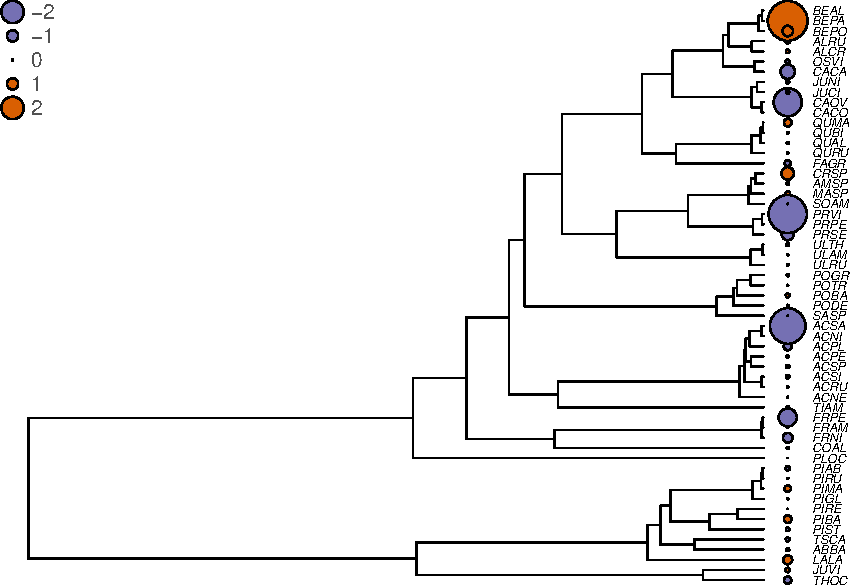
\includegraphics{pcm-workshop_files/figure-latex/Challenge 3 - solution-1.pdf}

\begin{Shaded}
\begin{Highlighting}[]
\FunctionTok{par}\NormalTok{(op)}
\end{Highlighting}
\end{Shaded}

\section{Défi 4}\label{duxe9fi-4}

Essayez d'ajuster un PGLS avec une structure de corrélation de Pagel en régressant la tolérance à l'ombre sur la masse des graines. Les résidus sont-ils aussi corrélés phylogénétiquement que dans la régression précédente avec la densité du bois~?

\begin{Shaded}
\begin{Highlighting}[]
\CommentTok{\# Ajuster un PGLS}
\NormalTok{Sm.pgls2 }\OtherTok{\textless{}{-}} \FunctionTok{gls}\NormalTok{(Shade }\SpecialCharTok{\textasciitilde{}}\NormalTok{ Sm, }\AttributeTok{data =}\NormalTok{ seedplantsdata, }\AttributeTok{correlation=}\NormalTok{pagel.corr)}
\CommentTok{\# Résultats}
\FunctionTok{summary}\NormalTok{(Sm.pgls2)}
\end{Highlighting}
\end{Shaded}

\begin{verbatim}
## Generalized least squares fit by REML
##   Model: Shade ~ Sm 
##   Data: seedplantsdata 
##        AIC      BIC    logLik
##   187.6889 195.7183 -89.84447
## 
## Correlation Structure: corPagel
##  Formula: ~Code 
##  Parameter estimate(s):
##   lambda 
## 0.951553 
## 
## Coefficients:
##                  Value Std.Error   t-value p-value
## (Intercept)  2.8204268  1.497276  1.883705  0.0649
## Sm          -0.0000716  0.000060 -1.193604  0.2378
## 
##  Correlation: 
##    (Intr)
## Sm -0.009
## 
## Standardized residuals:
##        Min         Q1        Med         Q3        Max 
## -0.6946682 -0.3115198  0.1068607  0.2604470  0.8319385 
## 
## Residual standard error: 2.620527 
## Degrees of freedom: 57 total; 55 residual
\end{verbatim}

  \bibliography{book.bib}

\end{document}
